\documentclass[a4paper]{article}
\usepackage[utf8]{inputenc}


%=-=-=-=-=-=-=-=-=-=-=-=-=-=-=-=-=-=-=-=-=-=-=-=-=-=-=-=-=-=-=-=-=-=-=-=-=-=-=-=-
% PREAMBLE
%=-=-=-=-=-=-=-=-=-=-=-=-=-=-=-=-=-=-=-=-=-=-=-=-=-=-=-=-=-=-=-=-=-=-=-=-=-=-=-=-

%%%%%%%%%%%%%%%%%%%%%%%%%%%%%%%%%%%%%%%%%%%%%%%%%%%%%%%%%%%%%%%%%%%%%
% Important styling notes
%%
% For now, to include img.jpg in img/path/to/img.jpg, just use:
% path/to/img.jpg - for details see style.tex
%=-=-=-=-=-=-=-=-=-=-=-=-=-=-=-=-=-=-=-=-=-=-=-=-=-=-=-=-=-=-=-=-=-=-=-=-=-=-=-=-
% Packages
%%
%\usepackage{fullpage} % Package to use full page
\usepackage[top=1in,bottom=1in,left=1in,right=1in,heightrounded]{geometry}

\usepackage{parskip}                    % Package to tweak paragraph skipping
\usepackage{amsmath}                    % standard
\usepackage{amssymb}                    % standard - Double R symbol etc.
\usepackage{hyperref}
\usepackage{amsthm}                     % standard - theorem, definition, etc.
\usepackage{multicol}                   % multiple columns for numbering
\usepackage{enumitem}                   % standard - enumerate styles
\usepackage[utf8]{inputenc}
\usepackage{scrextend}                  % indentation
\usepackage{graphicx}                   % standard - add figures
\usepackage{float}                      % standard - figure position, use [H] option
\usepackage{pifont}                     % symbols http://willbenton.com/wb-images/pifont.pdf
                                        % e.g. \ding{51}
\usepackage{gensymb}                    % degree symbol \degree
\usepackage{xcolor}                     % bg color
\hypersetup{
    colorlinks,
    linkcolor={black!50!black},
    citecolor={blue!50!black},
    urlcolor={blue!80!black}
}
\usepackage{framed}                     % bg color
\usepackage[T1]{fontenc}                % small caps
\usepackage{sectsty}                    % headings colour
\usepackage{mathtools}                  % Loads amsmath
\usepackage{amsthm,thmtools,xcolor}     % coloured theorem
\usepackage[toc,page]{appendix}         % reference to appendix
%\usepackage{titlesec}                   % change chapter, section, etc. formats
\usepackage{xifthen}                    % if, else
\usepackage{etoolbox}
% format numbering in theorem, lemma, etc. environment
\AtBeginEnvironment{theorem}{\setlist[enumerate, 1]{font=\upshape,  wide=0.5em, before=\leavevmode}}
\AtBeginEnvironment{lemma}{\setlist[enumerate, 1]{font=\upshape,  wide=0.5em, before=\leavevmode}}
\usepackage[letterspace=150]{microtype} % \textls{<letterspaced text>} % 0 <= letterspace <= 1000, 1000 = M space
\usepackage{letltxmacro}                % renew commands?
\usepackage{minted}                     % package to list code
    % otherwise minted goes off the page
    \setmintedinline{breaklines}
\usepackage{subfig}
\usepackage{eso-pic}                    % title page bg pic
\usepackage{varwidth}
\PassOptionsToPackage{svgnames}{xcolor}
\usepackage{fontawesome}                % \faQuestionCircle
\usepackage{marvosym}                   %\Pointinghand
\usepackage{mdframed}                   % easy outline frames
\usepackage[many]{tcolorbox}            % colour box for theorem styles
\usepackage{array,booktabs,calc} % table figs and text
\usepackage{comment}                    % \begin{comment}
\usepackage{fancyhdr}                   % page headings
\usepackage{mdframed}                   % boxes
\usepackage[backend=biber,sorting=none,style=ieee]{biblatex}
\usepackage{caption}
%%% caption options {
%\DeclareCaptionFont{white}{\color{white}}
\DeclareCaptionFormat{listing}{\colorbox{magenta!30!gray}{\parbox{\textwidth}{#1#2#3}}}
\captionsetup[lstlisting]{format=listing,labelfont={bf,small},textfont=small,skip=-1pt}
%%% }
\addbibresource{bibliography.bib}
\usepackage{url}
\usepackage{textcomp}
\usepackage[makeroom]{cancel}           % crossed symbols - \cancel{}, \bcancel{}, xcancel{}
\usepackage{algorithm}
\usepackage[noend]{algpseudocode}
\usepackage{tikz}
\usetikzlibrary{arrows.meta,positioning,quotes} % arrows and nodes in tikz
\usepackage{marginnote}                 % things in page margin by \marginnote{...}
\usepackage{pgfplots}
\usepackage{pstricks-add,pst-slpe}      % for fancy tikz arrows
%\usepackage{titlesec}                  % title style
\usepackage{lmodern}                    % a font
\usepackage{titletoc}                   % Required for manipulating the table of contents
\usepackage{titlesec}                   % Allows customization of titles
\usepackage{fouriernc}                  % Use the New Century Schoolbook font
\usepackage{booktabs}                   % better tables
\usepackage{stmaryrd }                  % \varoast
\usepackage{listings}                   % code listings
\usepackage{longtable}                  % table across multiple pages
\usepackage{todonotes}                  % TODO bubbles by \todo{...} command
\usepackage{changepage}                 % paragraph margins
\usepackage{tikz}
\usetikzlibrary{calc}
\usepackage{eso-pic}
\usepackage{transparent}



%=-=-=-=-=-=-=-=-=-=-=-=-=-=-=-=-=-=-=-=-=-=-=-=-=-=-=-=-=-=-=-=-=-=-=-=-=-=-=-=-
% Colours for various things
%%


\definecolor{shadecolor}{rgb}{1.,0.933,0.96} % bg color, r,g,b <= 1
\definecolor{medium_blue}{RGB}{60,125,190}
\definecolor{dark_blue}{RGB}{25,60,85}
\definecolor{dark_red}{RGB}{77,16,16}
\definecolor{LightPink}{rgb}{0.92.,0.8,0.84} % bg color, r,g,b <= 1
\definecolor{LighterPink}{rgb}{1.,0.94,0.97} % bg color, r,g,b <= 1
\definecolor{LightestPink}{rgb}{1.,0.95,0.99} % bg color, r,g,b <= 1
\definecolor{DarkestPink}{rgb}{0.36, 0.0, 0.18}
\definecolor{DarkerPink}{rgb}{0.41, 0.0, 0.21}
\definecolor{DarkPink}{rgb}{0.55, 0.05, 0.37}
\definecolor{lightestestpink}{RGB}{255,248,252}
\definecolor{codegray}{rgb}{0.5,0.5,0.5}
\definecolor{codegrayblue}{rgb}{0.35,0.35,0.47}



%=-=-=-=-=-=-=-=-=-=-=-=-=-=-=-=-=-=-=-=-=-=-=-=-=-=-=-=-=-=-=-=-=-=-=-=-=-=-=-=-
% Define my own theorem styles
%%

% "base" styles
\declaretheoremstyle[
  headfont=\color{DarkPink}\bfseries,
  bodyfont=\itshape,
]{colored}

\declaretheoremstyle[
  headfont=\color{DarkPink}\bfseries,
  bodyfont=\normalfont,
]{colored_upright}

% theorems (corollaries, etc) themselves, inherit from my style above
% Usage:
% \begin{theorem} \end{theorem}, \begin{lemma} \end{lemma}, ...
\declaretheorem[
	numberwithin=section,
 	style=colored,
	name=\textsc{Theorem},
]{theorem}

\tcolorboxenvironment{theorem}{
  boxrule=0pt,
  boxsep=2pt,
  colback={magenta!25!white},
  colframe=DarkPink,
  enhanced jigsaw, 
  borderline west={2pt}{0pt}{DarkPink},
  sharp corners,
  before skip=5pt,
  after skip=5pt,
  breakable,
  right=0mm % for equations
}

\declaretheorem[
	numberwithin=section,
 	style=colored,
	name=\textsc{Corollary},
]{corollary}

\tcolorboxenvironment{corollary}{
  boxrule=0pt,
  boxsep=1pt,
  colback={magenta!10!white},
  colframe=DarkPink,
  enhanced jigsaw, 
  borderline west={2pt}{0pt}{DarkPink},
  sharp corners,
  before skip=5pt,
  after skip=5pt,
  breakable,
  right=0mm % for equations
}

\declaretheorem[
	numberwithin=section,
	style=colored,
	name=\textsc{Lemma},
]{lemma}

\tcolorboxenvironment{lemma}{
  boxrule=0pt,
  boxsep=1pt,
  colback={magenta!10!white},
  colframe=DarkPink,
  enhanced jigsaw, 
  borderline west={2pt}{0pt}{DarkPink},
  sharp corners,
  before skip=5pt,
  after skip=5pt,
  breakable,
  right=0mm % for equations
}

\declaretheorem[
	numberwithin=section,
	style=colored,
	name=\textsc{Definition},
]{definition}

\tcolorboxenvironment{definition}{
  boxrule=0pt,
  boxsep=1pt,
  colback={magenta!25!white},
  colframe=DarkPink,
  enhanced jigsaw, 
  borderline west={2pt}{0pt}{DarkPink},
  sharp corners,
  before skip=5pt,
  after skip=5pt,
  breakable,
  right=0mm % for equations
}

\declaretheorem[
	numberwithin=section,
  	style=colored,
  	name=\textsc{Example},
]{exmp}

\declaretheorem[
	numberwithin=section,
  	style=colored,
  	name=\textsc{Solution},
]{soln}

%%% code listings
\lstdefinestyle{code1}{
    backgroundcolor=\color{lightestestpink},   
    commentstyle=\color{codegrayblue},
    keywordstyle=\color{DarkerPink},
    numberstyle=\tiny\color{codegray},
    stringstyle=\color{black!40!cyan},
    basicstyle=\small\ttfamily,
    breakatwhitespace=false,
    breaklines=true,        
    captionpos=t,             
    keepspaces=true,        
    numbers=left,           
    numbersep=5pt,
    showspaces=false, 
    showstringspaces=false,
    showtabs=false,
    tabsize=4
}

%%% code listings
\lstdefinestyle{code1}{
    backgroundcolor=\color{lightestestpink},   
    commentstyle=\color{codegrayblue},
    keywordstyle=\color{DarkerPink},
    numberstyle=\tiny\color{codegray},
    stringstyle=\color{black!40!cyan},
    basicstyle=\small\ttfamily,
    breakatwhitespace=false,
    breaklines=true,        
    captionpos=t,             
    keepspaces=true,        
    numbers=left,           
    numbersep=5pt,
    showspaces=false, 
    showstringspaces=false,
    showtabs=false,
    tabsize=4
}


\lstdefinestyle{terminal}{
    backgroundcolor=\color{black!5},   
    commentstyle=\color{codegrayblue},
    keywordstyle=\color{DarkerPink},
    %numberstyle=\tiny\color{codegray},
    stringstyle=\color{black!40!cyan},
    basicstyle=\small\ttfamily,
    numbers=none,
    breakatwhitespace=false,
    breaklines=true,        
    %captionpos=t,             
    keepspaces=true,        
    %numbers=left,           
    %numbersep=5pt,
    showspaces=false, 
    showstringspaces=false,
    showtabs=false,
    tabsize=4
}

\lstset{style=code1}

%=-=-=-=-=-=-=-=-=-=-=-=-=-=-=-=-=-=-=-=-=-=-=-=-=-=-=-=-=-=-=-=-=-=-=-=-=-=-=-=-
% Headers (size, font, colour)
%%

\makeatletter
\renewcommand{\@seccntformat}[1]{\llap{\textcolor{DarkestPink}{\csname the#1\endcsname}\hspace{1em}}}                    
\renewcommand{\section}{\@startsection{section}{1}{\z@}
{-4ex \@plus -1ex \@minus -.4ex}
{1ex \@plus.2ex }
{\normalfont\large\sffamily\bfseries\textcolor{DarkestPink}}}
\renewcommand{\subsection}{\@startsection {subsection}{2}{\z@}
{-3ex \@plus -0.1ex \@minus -.4ex}
{0.5ex \@plus.2ex }
{\normalfont\sffamily\bfseries\textcolor{DarkestPink}}}
\renewcommand{\subsubsection}{\@startsection {subsubsection}{3}{\z@}
{-2ex \@plus -0.1ex \@minus -.2ex}
{.2ex \@plus.2ex }
{\normalfont\small\sffamily\bfseries\textcolor{DarkestPink}}}                        


%=-=-=-=-=-=-=-=-=-=-=-=-=-=-=-=-=-=-=-=-=-=-=-=-=-=-=-=-=-=-=-=-=-=-=-=-=-=-=-=-
% Numberings, counters and spacings
%%
\numberwithin{equation}{section} % section number in eq/s
\setlength{\jot}{7pt} % spacing in split, gathered env/s



%% Custom examples
%% Output - Example 1,2,...
\newcounter{example}
\newenvironment{example}[1][]{\refstepcounter{example}\par\medskip
   \textbf{Example~\theexample. #1} \rmfamily}{\medskip}
%%%%%%%%%%%% End of unused %%%%%%%%%%%%



%=-=-=-=-=-=-=-=-=-=-=-=-=-=-=-=-=-=-=-=-=-=-=-=-=-=-=-=-=-=-=-=-=-=-=-=-=-=-=-=-
% Paths
%%

%=-=-=-=-=-=-=-=-=-=-=-=-=-=-=-=-=-=-=-=-=-=-=-=-=-=-=-=-=-=-=-=-=-=-=-=-=-=-=-=-
% User defined macros (math mode)
%%


% Curly braces under text. Usage: \myunderbrace{upper}{lower}
\newcommand{\myunderbrace}[2]{\mathrlap{\underbrace{\phantom{#1}}_{#2}} #1}
\newcommand{\setR}{\mathbb{R}} % \ouble R
\newcommand{\setRn}{\mathbb{R}^n} %  double R^n
\newcommand{\setN}{\mathbb{N}} % double N
\newcommand{\setZ}{\mathbb{Z}} % double Z
\let\oldemptyset\emptyset
\let\emptyset\varnothing % nice - looking empty set symbol
\newcommand{\fancyN}{\mathcal{N}} % null space
\newcommand{\fancyR}{\mathcal{R}} % range

\newcommand{\ba}{\textbf{a}}
\newcommand{\bw}{\textbf{w}}
\newcommand{\bx}{\textbf{x}}
\newcommand{\bu}{\textbf{u}}
\newcommand{\by}{\textbf{y}}
\newcommand{\bz}{\textbf{z}}
\newcommand{\bb}{\textbf{b}}
\newcommand{\bA}{\textbf{A}}
\newcommand{\bB}{\textbf{B}}
\newcommand{\bC}{\textbf{C}}
\newcommand{\bD}{\textbf{C}}
\newcommand{\bI}{\textbf{I}}
\newcommand{\bO}{\textbf{0}}
\newcommand{\bS}{\textbf{S}}
\newcommand{\bX}{\textbf{X}}
\newcommand{\bU}{\textbf{U}}
\newcommand{\bY}{\textbf{Y}}
% double bars as in norm
%\newcommand{\norm}[1] {\left|\left| #1 \right| \right|} 
\newcommand{\norm}[1]{\left\lVert#1\right\rVert}
\renewcommand{\t}{^{\top}}

\newcommand{\mean}[1]{\bar{#1}}
\newcommand{\var}{\sigma^2}

\newcommand{\partdevx}[1]{\frac{\partial #1}{\partial x}}
\newcommand{\partdevt}[1]{\frac{\partial #1}{\partial t}}
\newcommand{\partdevxx}[1]{\frac{\partial #1}{\partial x}}
\newcommand{\partdevxn}[1]{\frac{\partial^n #1}{\partial x^n}}
\newcommand{\partdevy}[1]{\frac{\partial #1}{\partial y}}
\newcommand{\partdevyy}[1]{\frac{\partial #1}{\partial y}}
\newcommand{\partdevyn}[1]{\frac{\partial^n #1}{\partial y^n}}

% text above = symbol
\newcommand{\overeq}[1]{\ensuremath{\stackrel{#1}=}} 
\newcommand{\greatersmaller}{%
  \mathrel{\ooalign{\raisebox{.6ex}{$>$}\cr\raisebox{-.6ex}{$<$}}}
} % greater and smaller symbols on top of each other, same line

%=-=-=-=-=-=-=-=-=-=-=-=-=-=-=-=-=-=-=-=-=-=-=-=-=-=-=-=-=-=-=-=-=-=-=-=-=-=-=-=-
% User defined macros (non math)

\newcommand{\qedblack}{$\hfill\blacksquare$} % black square end of line
\newcommand{\qedwhite}{\hfill \ensuremath{\Box}} % white square end of line
\newcommand{\hquad}{\hskip0.5em\relax}% half quad space
%\newcommand{\TODO}{\textcolor{red}{\bf TODO!}\;}

\newcommand{\TODO}[1][]{%
    \ifthenelse{\equal{#1}{}}{\textcolor{red}{\bf TODO!}\;}{\textcolor{red}{\textbf {TODO:} #1}\; }%
}
\newcommand{\B}[1]{\textbf{\textup{#1}}} % bold and upright
\renewcommand{\labelitemi}{\scriptsize$\textcolor{DarkPink}{\blacksquare}$} % itemize - squares instead of bullets
\newcommand{\emphasis}[1]{\textls{#1}}

\LetLtxMacro{\originaleqref}{\eqref}
\renewcommand{\eqref}{Eq.~\originaleqref}
\renewcommand*{\eqref}[1]{Eq.~\originaleqref{#1}}





% background images
%%%%%%%
\newcommand\BackgroundPic{%
\put(0,0){%
\parbox[b][\paperheight]{\paperwidth}{%
\vfill
%\centering
\includegraphics[width=0.125\paperwidth,height=\paperheight,%
]{img/background_02.png}% use ,keepaspectratio
\vfill
}}}
%%%%%%%
% end of background image
%%%%%%%%%%%%%% my own frame
\newmdenv[topline=false,bottomline=false]{leftrightbox}
%%%%%%%%%%%%% end
%%%%%%%%%%%%% my own comment
\newcommand{\mycomment}[1]{\begin{leftrightbox}\Pointinghand~\textbf{Comment:}~#1 \end{leftrightbox}}
%%%%%%%%%%%%% end
% my custom note https://tex.stackexchange.com/questions/301993/create-custom-note-environment-with-tcolorbox
\newmdenv[
    topline=false,
    bottomline=false,
    rightline=false,
    innerrightmargin=0pt
]{siderule}
\newenvironment{mynote}%
    {\begin{siderule}\textbf{\Pointinghand~Note:}}
    {\end{siderule}}
    
\newenvironment{myquote}%
    {\begin{adjustwidth}{0.4cm}{0.4cm}\faQuoteLeft\ \itshape}
    { \hfill \faQuoteRight  \end{adjustwidth}}
%%%%%%%%%%%%% my own box
\newcommand{\boxone}[1]{\begin{tcolorbox}[colback = LighterPink,colframe=LightPink]
#1
\end{tcolorbox}}
%%%%%%%%%%%%% end

\let\oldemptyset\emptyset
\let\emptyset\varnothing
%algorithmic
\algdef{SE}[DOWHILE]{Do}{doWhile}{\algorithmicdo}[1]{\algorithmicwhile\ #1}%

%%% otherwise minted goes off the page
\setmintedinline{breaklines}





\begin{document}
%=-=-=-=-=-=-=-=-=-=-=-=-=-=-=-=-=-=-=-=-=-=-=-=-=-=-=-=-=-=-=-=-=-=-=-=-=-=-=-=-
% GLOBAL STYLES (DOCUMENT SCOPE)
%=-=-=-=-=-=-=-=-=-=-=-=-=-=-=-=-=-=-=-=-=-=-=-=-=-=-=-=-=-=-=-=-=-=-=-=-=-=-=-=-
% caption: Figure 1 -> <bold> Fig. 1 </bold>
\captionsetup[figure]{labelfont={bf},labelformat={default},labelsep=period,name={Fig.}}


%=-=-=-=-=-=-=-=-=-=-=-=-=-=-=-=-=-=-=-=-=-=-=-=-=-=-=-=-=-=-=-=-=-=-=-=-=-=-=-=-
% TITLE PAGE
%=-=-=-=-=-=-=-=-=-=-=-=-=-=-=-=-=-=-=-=-=-=-=-=-=-=-=-=-=-=-=-=-=-=-=-=-=-=-=-=-
%%%%%%%%%%%%%%%%%%%%%%%%%%%%%%%%%%%%%%%%%
% Formal Book Title Page
% LaTeX Template
% Version 2.0 (23/7/17)
%
% This template was downloaded from:
% http://www.LaTeXTemplates.com
%
% Original author:
% Peter Wilson (herries.press@earthlink.net) with modifications by:
% Vel (vel@latextemplates.com)
%
% License:
% CC BY-NC-SA 3.0 (http://creativecommons.org/licenses/by-nc-sa/3.0/)
% 
% This template can be used in one of two ways:
%
% 1) Content can be added at the end of this file just before the \end{document}
% to use this title page as the starting point for your document.
%
% 2) Alternatively, if you already have a document which you wish to add this
% title page to, copy everything between the \begin{document} and
% \end{document} and paste it where you would like the title page in your
% document. You will then need to insert the packages and document 
% configurations into your document carefully making sure you are not loading
% the same package twice and that there are no clashes.
%
%%%%%%%%%%%%%%%%%%%%%%%%%%%%%%%%%%%%%%%%%

%----------------------------------------------------------------------------------------
%	PACKAGES AND OTHER DOCUMENT CONFIGURATIONS
%----------------------------------------------------------------------------------------



%----------------------------------------------------------------------------------------
%	TITLE PAGE
%----------------------------------------------------------------------------------------



\begin{titlepage} % Suppresses headers and footers on the title page

    
   	%------------------------------------------------
	%	Text alignment
	%------------------------------------------------
	\centering % Centre everything on the title page
	
	\scshape % Use small caps for all text on the title page
	
	\vspace*{\baselineskip} % White space at the top of the page
	
	%------------------------------------------------
	%	Title
	%------------------------------------------------
	
	\rule{\textwidth}{1.6pt}\vspace*{-\baselineskip}\vspace*{2pt} % Thick horizontal rule
	\rule{\textwidth}{0.4pt} % Thin horizontal rule
	
	\vspace{0.75\baselineskip} % Whitespace above the title
	
	{\LARGE SHAPE RASTERISATION\\ \Large ALGORITHMS\\} % Title
	
	\vspace{0.75\baselineskip} % Whitespace below the title
	
	\rule{\textwidth}{0.4pt}\vspace*{-\baselineskip}\vspace{3.2pt} % Thin horizontal rule
	\rule{\textwidth}{1.6pt} % Thick horizontal rule
	
	\vspace{2\baselineskip} % Whitespace after the title block
	
	%------------------------------------------------
	%	Subtitle
	%------------------------------------------------
        Contents
	
	\vspace*{3\baselineskip} % Whitespace under the subtitle
	
        Straight Lines\\
        Curvy Lines\\
        Triangle Fill\\
        Circle Drawing
	
	\vspace*{3\baselineskip} % Whitespace under the subtitle
	
	%------------------------------------------------
	%	Editor(s)
	%------------------------------------------------
	
	By
	
	\vspace{0.5\baselineskip} % Whitespace before the editors
	
	{\normalfont \Large \mintinline{latex}{0xLeo} (\url{github.com/0xleo}) \\} % Editor list
	
	\vspace{0.5\baselineskip} % Whitespace below the editor list
	
	%\textit{The University of California \\ Berkeley} % Editor affiliation
	
	\vfill % Whitespace between editor names and publisher logo
	
	%------------------------------------------------
	%	Publisher
	%------------------------------------------------
	
	
	\vspace{0.3\baselineskip} % Whitespace under the publisher logo
	
	\today % Date
	
	{DRAFT X.YY} % Draft version
	{\\Missing: \ldots}

\end{titlepage}

%----------------------------------------------------------------------------------------

%\maketitle



%=-=-=-=-=-=-=-=-=-=-=-=-=-=-=-=-=-=-=-=-=-=-=-=-=-=-=-=-=-=-=-=-=-=-=-=-=-=-=-=-
% MAIN DOCUMENT
%=-=-=-=-=-=-=-=-=-=-=-=-=-=-=-=-=-=-=-=-=-=-=-=-=-=-=-=-=-=-=-=-=-=-=-=-=-=-=-=-
\newpage
\tableofcontents
\newpage



%------------------------------ New section ------------------------------%
\section{Ordinary Differential Equation Applications}

\subsection{Basic definitions}
% ref https://www.octawian.ro/fisiere/situri/edi/build/html/_downloads/b4227196c266cc7fd4e783895e5d00cb/Tenenbaum_Pollard.pdf
\begin{definition}[ODE]
    If $f(x)$ is a function defined at an interval $I:\; a < x < b$, then by \emphasis{ordinary differential equation} (ODE) we mean an equation involving $x$, the function $f(x)$ and one or more of its derivatives.
\end{definition}
We often denote $y:=f(x)$ so the following are ODEs:
\begin{gather*}
\frac{dy}{dx} + y = 0 \\
f''(x) = -4f'(x) \\
y^{(4)} + 2x y'' = x^3
\end{gather*}
% ref https://tutorial.math.lamar.edu/classes/de/separable.aspx




\subsection{Separable ODEs}

\begin{definition}[separable ODE]
An ODE that can be written in the form
\begin{equation}
    N(y)\frac{dy}{dx} = M(x)
    \label{eq:def_separable}
\end{equation}
    is called \emphasis{separable}.
\end{definition}
\begin{corollary}[separable ODE]
   A separable ODE can be rewritten in the form
    \begin{equation}
        N(y)dy = M(x)dx
        \label{eq:ode_separable}
    \end{equation}
\end{corollary}
\begin{proof}
    To solve \eqref{eq:def_separable}, we integrate both sides w.r.t. $x$:
    \[
    \int N(y)\frac{dy}{dx} \; dx = \int M(x)\; dx
    \]
    Remember that by $y$ we denote a function of $x$, i.e. $y = y(x)$. Therefore letting:
    \[
    u:=y(x) \Rightarrow du = y'(x)dx = \frac{dy}{dx}dx
    \]
    , the integrals can be rewritten as:
    \[
    \int N(u)\; du = \int M(x)\; dx
    \]
    Because $u$ is a dummy variable, this is equivalent to: \[ \int N(y)\; dy = \int M(x)\; dx \]
    The takeaway is that to solve \eqref{eq:def_separable}, we can pretend that the derivative  $\tfrac{dy}{dx}$ is a fraction and that we can multiply both sides by $dx$.
\end{proof}
If an ODE is in the form:
\[
    f(x)dx + g(y)dy = 0
\]
, then we can integrate to find either an implicit (e.g. $x\, \cos(y) + 4x^3 - 1 = 0$) or an explicit (e.g. $y = -ln\, x$) solution. Whether the solution is implicit or explicit depends on whether $f(x)$ and $g(x)$ can be integrated.
\begin{exmp}[no initial condition]
% ref https://www.cliffsnotes.com/study-guides/differential-equations/first-order-equations/separable-equations 
Solve the equation
    \[
        x\, dx + \frac{\sin y}{\cos x}\, dy = 0
    \]
\end{exmp}
\begin{soln}
    Rewrite in the same form as \eqref{eq:ode_separable}:
    \[
    x\, \cos x \, dx + \sin y dy = 0
    \]
    Integrate both terms. Integrate the left term by parts:
    \begin{align*}
        & \int x \, \cos x \, dx  \\
        &= \int x \, (\sin x)' \, dx \\
        &= x\, \sin x + \int \sin x \, dx \\
        &= x\, \sin x - \cos x  + C
    \end{align*}
    , where $C$ is an arbitrary constant. Integrate the right term:
    \[
        \int \sin y \, dy = - \cos y + C
    \]
    , where $C$ is another arbitrary constant. Substitute both integrals to express the solution in a closed form:
    \[
        x\, \sin x - \cos x -\cos y  + C = 0
    \]
\end{soln}


\begin{exmp}[initial condition]
% ref https://www.cliffsnotes.com/study-guides/differential-equations/first-order-equations/separable-equations
Solve the ODE
    \[
        \frac{dy}{dx} = \frac{x(x^{x^2} + 2)}{6y^2} 
    \]
given that $y(0) = 1$.
\end{exmp}
\begin{soln}
Rewrite it as a separable equation:
    \[
        6y^2\, dy = x(e^{x^2} + 2)dx
    \]
Integrate both sides:
\begin{align*}
        \int 6y^2\, dy = \int x(e^{x^2} + 2) \, dx \Rightarrow
        2y^3 = \frac{1}{2} e^{x^2} + x^2 + C
\end{align*}
Set $x=0, \; y=1$ to determine $C$:
    \[
        2= 1/2 + C \Rightarrow C = 3/2
    \]
Therefore the (implicit) solution is:
    \[
        2y^3 = \frac{1}{2} e^{x^2} + x^2 + \frac{3}{2} 
    \]
\end{soln}

\begin{exmp}[dividing by zero]
Solve the ODE
    \[
        \frac{dy}{dx} = (1 + e^{-x})(y^2 - 1)
    \]
\end{exmp}
\begin{soln}
To separate the equation, we have to divide by $(y^2-1)$. However, that maybe be zero for certain values of $y$. Therefore before we divide by it, we have to exclude those values first and test them (manually) in a separate step.

For starters, divide by $(y^2 - 1)$ for $(y^2 - 1) \neq 0$, i.e. $y \neq 1$ and $y \neq -1$.

    \[
        \frac{dy}{y^2 - 1} = (1 + e^{-x})  \, dx
    \]
Integrate it:
\begin{align*}
    \int \frac{dy}{y^2 - 1} = \int (1 + e^{-x})  \, dx \Rightarrow \\
    \int \Bigg(\frac{-\frac{1}{2}}{y+1} + \frac{\frac{1}{2}}{y-1}\Bigg)\, dy = \int (1 + e^{-x})  \, dx \Rightarrow \\
    \ln \left| \frac{y-1}{y+1} \right| = 2(x-e^{-x} + C) \tag{\ding{78}}
    \label{eq:ode_sep_ex3}
\end{align*}
\end{soln}
$\eqref{eq:ode_sep_ex3}$ describes a solution to the original ODE. However we have excluded $y = \pm 1$ so we need to test these too. For $y=\pm 1$, the original ODE yields a statement that is true for any $x$:
\[
    0 = (1 + e^{-x})(1 - 1)
\]
Therefore the family
\[
   y = \pm 1  \tag{\ding{78}\ding{78}}
\]
is also a solution.



\subsubsection{Separable Equations and Substitution Methods}

The theory of separable equations can be applies to solve first-order ODEs of the form $\tfrac{dy}{dx} = F(ax + by + c)$.
\begin{corollary}
The substitution $v=ax+by+c$ transforms the equation
\begin{equation}
\frac{dy}{dx} = F(ax+by+c)
\end{equation}
into a separable equation.
\end{corollary}
\begin{proof}
% ref https://www.math.bgu.ac.il/~nicola/courses/ode/Ionascu_LectNotes.pdf p17
Let's assume $b\neq 0$. Using the substitution $v=ax+by+c$ and differentiating w.r.t. $\tfrac{dv}{dx} = a + b\tfrac{dy}{dx}$, then the equation becomes:
\[
\frac{dv}{dx} = a + bF(v) \Rightarrow \frac{dv}{a+F(v)} = dx
\]
The latter equation is separable.

If $b=0$, then the equation $\tfrac{dy}{dx} = F(ax + c)$ is already separable.
\end{proof}

\subsubsection{Application: Newton's Law of Cooling}

% ref https://www.math.bgu.ac.il/~nicola/courses/ode/Ionascu_LectNotes.pdf p.13
Newton's law of cooling describes the temperature of a hot body if it immersed in a medium of constant temperature \footnote{Newton's law of cooling can be derived if we take into account the rate of \textit{net} heat transfer by radiation equation (a.k.a. Stefan-Boltzmann law): $dQ =  eA\sigma(T^4 - T_0^4)$ and the fundamental law of thermodynamics: $Q = msT \Rightarrow dQ = ms \, dT$}, e.g. a thermos of warm coffee in a room. More concretely, ``the time rate of change of the temperature $T(t)$ of a body of initial temperature $T_0$ immersed in a medium of constant temperature M is proportional to the difference $M - T (t)$''. This translates into:
\begin{equation*}
    T'(t) = k\left(M - T(t) \right)
\end{equation*}
\eqref{eq:newtons_law_cooling} is separable as it can be rewritten as (assuming hot body, therefore $T(t)> M\; \forall t$):
\begin{gather*}
    \frac{T'(t)}{T(t) - M} = -k  \Rightarrow \\
    \ln\left|T(t) - M \right| = \ln\left( T(t) - M \right) = -kt + C \Rightarrow \\
    T(t) = e^{-kt}e^C + M
\end{gather*}
We know $T(0) = T_0$, so plugging $t=0$ in the latter equation we obtain:
\[
   e^C = T_0 - M 
\]
To summarise.
\begin{corollary}[Newton's law of cooling]
Assuming $T(t) > M$, the solution to the DE 
\begin{equation}
    T'(t) = k\left(M - T(t) \right)
    \label{eq:newtons_law_cooling}
\end{equation}
, where $k$ and $M$ are constants, is given by:
\begin{equation}
    T(t) = M + e^{-kT}(T(0) - M)
    \label{eq:newtons_law_cooling_sol}
\end{equation}
\end{corollary}



\subsection{Homogeneous ODEs}
% https://www.cliffsnotes.com/study-guides/differential-equations/first-order-equations/first-order-homogeneous-equations
\begin{definition}[homogeneous function]
% ref https://www.cliffsnotes.com/study-guides/differential-equations/first-order-equations/first-order-homogeneous-equations
A function $f(x,y)$ is said to be homogeneous of degree $n$ if the equation
\begin{equation}
    f(zx, zy) = z^n f(x,y) 
\end{equation}
holds for all $x,y$ and $z$ (for which both sides are defined).
\end{definition}
% https://www.math.bgu.ac.il/~nicola/courses/ode/Ionascu_LectNotes.pdf
% https://www.mathsisfun.com/calculus/differential-equations-homogeneous.html
\begin{exmp}
Prove that the function $f(x,y) = x^2 + y^2 - xy$  is homogeneous and find its degree.
\end{exmp}
\begin{soln}
    \[
        f(zx,zy) =(zx)^2 + (zx)^2 - zx\cdot zy   = z^2(x^2 + y^2 - xy) = z^2 f(x,y)
    \]
Therefore its degree is 2.
\end{soln}

\begin{definition}[homogeneous ODE]
% ref https://www.cliffsnotes.com/study-guides/differential-equations/first-order-equations/first-order-homogeneous-equations 
    A first‐order ODE  is said to be \emphasis{homogeneous} if $M(x,y)$ and $N(x,y)$ are both homogeneous functions of the same degree.
\label{def:ode_homo}
\end{definition}
Homogeneous ODEs of first order can be solved by setting
\begin{gather}
    v = \frac{y}{x} \Rightarrow y = vx \label{eq:ode_sep_yvx} \\
    \therefore \frac{dy}{dx} = \frac{d(vx)}{dx} \nonumber \\
    \therefore \frac{dy}{dx} = v + x \frac{dv}{dx}  \label{eq:ode_sep_dy}
\end{gather}


% TODO: https://www.cliffsnotes.com/study-guides/differential-equations/first-order-equations/first-order-homogeneous-equations ex. 7 or
% https://math24.net/separable-equations.html

\begin{exmp}
Solve $x^2 - y^2 + 2xyy' = 0$
\end{exmp}
\begin{soln}
It can be rewritten as:
    \[
        \underbrace{(x^2  -y^2)}_{M(x,y)} \, dx + \underbrace{2xy}_{N(x,y)}\, dy = 0
    \]
    $M(x,y)$ and $N(x,y)$ are both homogeneous functions of degree 2 as $M(zx, zy) = z^2 M(x,y)$ and $N(zx, zy) = z^2 N(x,y)$ therefore the DE is homogeneous of degree 2. To solve it by making it separable, the substitutions in \eqref{eq:ode_sep_yvx}, \eqref{eq:ode_sep_dy} can be applied. However before applying them, divide first by $x^2$ (for $x\neq 0$) to show up the ratio $y/x$:
    \[
        1 - \left(\frac{y}{x} \right)^2 + 2 \frac{y}{x} y' = 0
        \label{eq:ode_sep_ex1_yx}
        \tag{\ding{78}}
    \]
    Now apply the transform in  in \eqref{eq:ode_sep_yvx}, \eqref{eq:ode_sep_dy}:
    \[
    y=vx, \quad \frac{dy}{dx}  = v + x \frac{dv}{dx} 
    \]
    \eqref{eq:ode_sep_ex1_yx} becomes:
    \begin{gather*}
        1 - v^2 + 2v(v + xv')= 0 \Rightarrow \\
        1 + v^2 + 2xvv'  = 0 \Rightarrow \\
        \frac{2vv'}{1 + v^2} =  - \frac{1}{x} \Rightarrow \\ 
        \ln(1+v^2) = -\ln x + C  = \ln(\frac{C}{x})\Rightarrow \\
        (1 + v^v2)x = A 
    \end{gather*}
    , where $A$ is another arbitrary constant such that $\ln C = A$. Substituting back $v$ with $y/x$:
    \begin{gather*}
        x + \frac{y^2}{x} = A \Rightarrow \\
        y^2 = Ax - x^2 \Rightarrow \\
        y = \pm \sqrt{Ax - x^2} \label{eq:ode_sep_ex1_sol1} \tag{\ding{78}\ding{78}}
    \end{gather*}
    This solution holds for $x \neq 0$. Testing for $x=0$:
    \[
    y = 0 
    \]
    Hence the point $(0,0)$ and \eqref{eq:ode_sep_ex1_sol1} are all the solutions.
\end{soln}

\begin{exmp}
    % ref https://www.math.bgu.ac.il/~nicola/courses/ode/Ionascu_LectNotes.pdf p.19
    Find the solution(s) of the homogeneous ODE  
\[
    yy' + x = \sqrt{x^2 + y^2}, \quad x, y > 0
\]
\end{exmp}
\begin{soln}
    The equation can be rewritten:
    \begin{gather*}
        y\, dy + x\, dx = \sqrt{x^2 + y^2} \, dx \Rightarrow \\
        \underbrace{y}_{M(x)}\, dy = \underbrace{(\sqrt{x^2 + y^2} - x)}_{N(x,y)}\, dx
    \end{gather*}
    It's easy to see (Def'n \ref{def:ode_homo}) that the latter is homogeneous of degree 1, as both $M(x,y), \, N(x,y)$ have the same degree of 1. Set $y=vx \Rightarrow y' = v + x \tfrac{dv}{dx} = v+xv'$. Then the equation becomes (we eliminate $y$):
    \begin{gather*}
        xv \, \left(v + x v'\right)  + x = \sqrt{x^2(1+v^2)}\, dx = x\sqrt{1+v^2} \, dx \Rightarrow \\
        v\left(v + xv'\right) = \sqrt{1 + v^2} - 1 \Rightarrow \\
        xvv' = \sqrt{1 + v^2} - 1 - v^2
    \end{gather*}
    $y,x > 0 \therefore v > 0$ so we can divide:
    \begin{gather*}
        \frac{vv'}{v^2 + 1 - \sqrt{1 + v^2}}  = -\frac{1}{x}  \Rightarrow \\
        \frac{vv'}{\sqrt{v^2 + 1}(\sqrt{v^2 + 1} -1)}
    \end{gather*}
    We can multiply the LHS by the conjugate $(\sqrt{1+u^2} + 1)$ to simplify it:
    \begin{gather*}
        \frac{v(\sqrt{1+v^2} + 1)v'}{v^2\sqrt{1+v^2}} = -\frac{1}{x}   
    \end{gather*}
    This is already  a separable DE but at the moment it cannot be integrated. Break the fraction to make the LHS integrateable:
    \begin{gather*}
        \frac{v'}{v} + \frac{v'}{v\sqrt{1+v^2}} = -\frac{1}{x}  
    \end{gather*}
    Integrate both sides w.r.t $x$:
    \begin{gather*}
        \ln(v) + \int \frac{dv}{v\sqrt{1+v^2}} = -\ln x + C 
        \tag{\ding{72}}
        \label{eq:ode_hom_ex1}
    \end{gather*}
    To compute the remaining integral, change variables by setting $u = 1/v \Rightarrow dv = -du/u^2$:
    \begin{gather*}
        \int \frac{dv}{v\sqrt{1+v^2}} = -\int \frac{u}{\sqrt{1+ \tfrac{1}{u^2}}} \frac{du}{u^2}  = - \int \frac{du}{\sqrt{1+u^2}}  \\
        = -\ln \left|u + \sqrt{1+u^2} \right| + C' = -\ln\left|u\right| + \ln\left|\sqrt{1+u^2} + 1 \right| + C'
    \end{gather*}
    Plugging in the integral in \eqref{eq:ode_hom_ex1} we get:
    \begin{gather*}
        \ln\left|\sqrt{1+u^2} + 1 \right| = \ln \frac{1}{x} + \ln{K} = \ln \frac{K}{x}
    \end{gather*}
    , where $K$ is some other arbitrary non-negative constant such that $\ln K = C'$. Therefore, since $x>0$:
    \begin{gather*}
        \sqrt{1+u^2} + 1 = K/x \Rightarrow \\ 
        \frac{xv^2}{\sqrt{1+v^2} + 1} = K  \Rightarrow \\
        \frac{xv^2(\sqrt{1+v^2} - 1)}{v^2} = x(\sqrt{1+v^2} - 1) = K
    \end{gather*}
    Since $v = y/x$, we obtain:
    \begin{gather*}
        x\left(\sqrt{1+\tfrac{y^2}{x^2}} - 1\right) = \sqrt{x^2 - y^2} - x = K \Rightarrow \\
    \end{gather*}
    Solving for $y(x)$:
    \[
        y(x) = \sqrt{(2x+K)K}, \quad x\in (-K/2, \infty)
    \]
    We obtained the last constraint since $(2x+K)$ is under the square root, therefore $2x+K\geq 0$. Additionally, the square root is positive as $y(x) > 0$.
\end{soln}



\subsection{Linear Differential Equations of First Order}

% ref https://math24.net/linear-differential-equations-first-order.html
\begin{definition}[linear non-homogeneous DE of first order] A differential equation of the type
    \begin{equation}
        y' + a(x)y = f(x)
        \label{eq:linear_de_first_order}
    \end{equation}
    , where $a(x)$ and $f(x)$ are continuous functions of $x$, is called linear non-homogeneous (NH) DE of first order. 
\end{definition}
Linear NH DEs of first order are typically solved by the method of integrating factor. If we multiply both sides of \eqref{eq:linear_de_first_order} by the factor $u(x) := \exp\left(\int a(x)\, dx\right)$, then it becomes:
\begin{gather*}
        \exp\left(\int a(x)\, dx\right)y' + \exp\left(\int a(x)\, dx\right)'y = f(x)\exp\left(\int a(x)\, dx\right) \Rightarrow \\
        u(x)y' + u'(x)y = f(x)u(x) \Rightarrow \\
        (u(x)y)' = f(x)u(x)  \Rightarrow \\
        y = \frac{\int f(x)u(x)\, dx + C}{u(x)} 
\end{gather*}
, where $C$ is an arbitrary constant. To summarise:
\begin{corollary}[solution of NH DE of first 1 order by intergrating factor]
    The solution of the DE
    \begin{equation}
        y' + a(x)y = f(x)
        \label{eq:nonhomo_first_order}
    \end{equation}
    is given in terms of the \emphasis{integrating factor} $u(x) =  \exp\left(\int a(x)\, dx\right)$ as:
    \begin{equation}
        y = \frac{\int f(x)u(x)\, dx + C}{u(x)} , \quad  u(x) =  \exp\left(\int a(x)\, dx\right)
        \label{eq:ide_nh_first_order_intergrating_factor}
    \end{equation}
    , where $C$ is an arbitrary constant.
\end{corollary}
Constant $C$ can be determined if we are given an initial condition $y(x_0) = y_0$.


\subsection{Exact equations}
Exact equations are a subset of the general first order DEs. They can easily be recognised and solved in some standard steps.
\begin{definition}[exact DE]
% ref weiglhofer, lindsay p4
A DE of type 
\begin{equation}
    P(x,y)dx + Q(x,y)dy = 0
    \label{eq:de_p_q}
\end{equation}
    , or equivalently $P(x,y) + Q(x,y)y' = 0$ is said to be \emphasis{exact} if there exists a function of two variables $u(x,y)$ with continuous partial derivatives such that:
    \begin{equation}
        \frac{\partial u}{\partial x} = P(x,y), \quad \frac{\partial u}{\partial y} = Q(x,y)
        \label{eq:de_exact_u}
    \end{equation}
\end{definition}

\begin{corollary}
Because of \eqref{eq:de_exact_u}, the general solution of an exact DE can be written in terms of the general solution as:
    \[
    \frac{\partial u}{\partial x}  + \frac{\partial u}{\partial y}  \frac{\partial y}{\partial x} = 0
    \]
    In other words, the \textit{total derivative} of $u(x,y)$ must be zero. Therefore any function $u(x,y) = C$, where $C$ is a constant, satisfies the DE.
\end{corollary}
From the interchangeability of the order of the partial derivatives, it also follows that the following condition is necessary for the \eqref{eq:de_p_q} to be exact.
\begin{corollary}[exactness conditions]
If 
\begin{equation}
    \frac{\partial P(x,y)}{\partial y}  = \frac{\partial Q(x,y)}{\partial x}
\end{equation}
, then the DE 
\begin{equation}
    P(x,y)dx + Q(x,y)dy = 0
    \label{eq:condition_exactness}
\end{equation}
is exact.
\end{corollary}
Exact DEs of the form \eqref{eq:de_p_q} can be solved in a certain recipe.
\begin{enumerate}
    \item (Test for exactness) Check whether the condition in \eqref{eq:condition_exactness}  is true:
        \[
            \frac{\partial P}{\partial y}   = \frac{\partial Q}{\partial x} 
        \]
    \item (Define the general solution function $u(x,y)$) Write the system
    \begin{gather*}
        \left\{
        \begin{array}{ll}
            \frac{\partial u}{\partial x}  = P(x,y) \\
            \frac{\partial u}{\partial y}  = Q(x,y)
        \end{array} 
        \right. 
    \end{gather*}
    
    \item \marginnote{When we integrate $u(x,y)$ w.r.t. $x$, we treat $y$ as a constant, hence the int. constant $\phi$ will be a function $y$.}(Integrate w.r.t $x$) Integrate the first equation w.r.t. $x$ or the second w.r.t. $y$ (whatever is easier). Without loss of generality, we proceed in the first way. Because we integrate w.r.t. $x$, instead of constant $C$ we have an unknown function of $y$:
        \[
            u(x,y) = \int P(x,y)\, dx + \phi(y)
            \tag{2}
        \]
        To find $u(x,y)$, we first need to determine $\phi(y)$.

    \item (Differentiate w.r.t. $y$ to determine the int. constant) From the exactness condition, we know $u_y = Q(x,y)$. Differentiate Eq. (2) w.r.t. $y$ to show up $\phi'(y)$:
        \begin{gather*}
            \frac{du}{dy} = \frac{\partial}{\partial y} \left[\int P(x,y)\, dx + \phi(y) \right] = Q(x,y) \Rightarrow \\
            \phi'(y) = Q(x,y) - \frac{\partial}{\partial y} \left(\int P(x,y)\, dx \right)
        \end{gather*}

    \item \marginnote{Don't need an int. constant here -- the general solution includes one.}(Determine int. constant)Integrating the last equation w.r.t. $y$ we can determine $\phi(y)$:
        \[
            \phi(y) = \int Q(x,y)\, dy - \int P(x,y) \, dx
            \tag{3}
        \]
        Plugging Eq. (3) in Eq. (2), we can determine $u(x,y)$.

    \item (Obtain the general solution) The general solution is written in closed form as:
        \[
            u(x,y) = C
        \]
\end{enumerate}

\begin{exmp}
% ref https://www.youtube.com/watch?v=AMqlalkGN8A
Consider the equation
    \[
        (2x + y) + (x + 2y)y' = 0
    \]
Is it exact? If so, find the solution given the initial condition $y(1) = 1$.
\end{exmp}
\begin{soln}
We have $P(x,y) = 2x+y$, $Q(x,y) = x + 2y$. $P_y = 1 = Q_x$ therefore is it exact.
    To solve it, we need to find a function $u(x,y)$ such that:
    \[
        u(x,y)_x = P(x,y) = 2x + y, \quad u(x,y)_y = Q(x,y) = x + 2y 
        \label{eq:exact_ex_1_1}
        \tag{\ding{78}}
    \]
    Integrate the first equation (w.r.t.) $x$:
    \[
        u(x,y) = \int u_x(x,y)\, dx = \int (2x + y) dx = x^2 + xy + \phi(y)
        \label{eq:exact_ex_1_2}
        \tag{\ding{78}\ding{78}}
    \]
    Differentiate \eqref{eq:exact_ex_1_2} w.r.t. $y$ and use \eqref{eq:exact_ex_1_1}:
    \begin{gather*}
        u_x(x,y) = x + \phi'(y) = x + 2y \Rightarrow\\
        \phi'(y) = 2y \Rightarrow \\
        \phi(y) = y^2
    \end{gather*}
    Therefore from \eqref{eq:exact_ex_1_2} we can determine $u(x,y)$: 
    \[
        u(x,y) = x^2 + xy + \phi(y) = x^2 + xy + y^2 
    \]
    The general solution is written in implicit form as:
    \[
        u(x,y) = C \Leftrightarrow x^2  +xy + y^2 = C
    \]
    , where $C$ is a constant that can be determined from the initial condition. The initial condition demands $y=1$ for $x=1$, therefore we can plug these in to obtain $C=3$. Therefore the implicit solution is:
    \[
        x^2  +xy + y^2 = 3
    \]
\end{soln}

\begin{exmp}
% ref https://www.youtube.com/watch?v=AMqlalkGN8A
Given the equation 
    \[
        (xy^2 + bx^2y) + (x+y)x^2 y' = 0
    \]
\begin{enumerate}
    \item Find the values of $b$ such that the equation is exact.
    \item Solve it with that value of $b$.
\end{enumerate}
\end{exmp}
\begin{soln}
\quad \\
   \begin{enumerate}
       \item We have
           \begin{gather*}
               P(x,y) = xy^2 + bx^2y, \quad Q(x,y) = x^3 + x^2y
               \therefore P_y = 2xy + bx^2, \quad Q_x = 3x^2 + 2xy
           \end{gather*}
        $P_y$ and $Q_x$ must be equal for the equation to be exact therefore $b=3$.

        \item For $b=3$, the partial derivatives of the solution are:
            \[
                u_x = P(x,y) = xy^2 + 3x^2y, \quad u_y = Q(x,y) = x^3 + x^2y
            \]
            Integrate the first equation w.r.t. $x$:
            \[
                u(x,y) = \int(xy^2 + 3x^2y)dx + h(y) = \frac{1}{2} x^2y^2 + x^3y + \phi(y)
            \]
            Differentiate the latter w.r.t. $y$ and use the exactness condition (remember, we don't need a constant at this stage so in the end we take $h(y) = 0$):
            \[
                u_x = x^2y + x^3 + \phi'(y) = x^3  +x^2y \Rightarrow \phi'(y) = 0 \Rightarrow h(y) = 0
            \]
            The implicit solution is:
            \[
                u(x,y) = C \Leftrightarrow \frac{1}{2} x^2y^2 + x^3y = C
            \]
   \end{enumerate} 
\end{soln}


\subsection{Application 2: Lake Pollution Model}

First order differential equations can be applied to model the pollution in a lake in a simplistic way. In the lake pollution problem, a lake is polluted by a stream of water (input), has an outflow (output) and the goal is to find the concentration (mass/volume) of the pollutant in the lake at any time.

We make the following assumptions before we describe the model:
\begin{itemize}
    \item \marginnote{Sometimes $c, c_{in}$ are measured in parts per $m^3$ but we'll stick to kg.}The pollutant is flowing in the lake has a concentration of $c_{in}(t)$ ($kg/m^3$) and flows in at a volumetric flow ($m^3/day$) of $f(t)$. 
    \item The lake is well-mixed, i.e. its pollutant concentration $c(t)$ ($kg/m^3$) is uniform.
    \item The lake maintains a constant volume $V$ ($m^3$) by having $\textup{outflow} = \textup{inflow} = f(t)$ ($m^3/day$).
\end{itemize}
Consequently, the mass of the pollutant in the lake $M(t)$ at any time is equal to:
\[
    M(t) = c(t)\cdot V 
    \tag{1}
\]
From the conservation of the mass of the pollutant, the system can be described in high level as:
\[
   \left \{ \begin{array}{c}
      \textup{rate\;  of \; change} \\
      \textup{of \; mass} \\
      \textup{of\;  pollutant} \\
      \textup{in\;  lake}
   \end{array} \right \}
   = 
      \left \{ \begin{array}{c}
      \textup{rate \; at} \\
      \textup{which \; the} \\
      \textup{pollutant \; enters} \\
      \textup{the \; lake} 
   \end{array} \right \} - 
      \left \{ \begin{array}{c}
      \textup{rate \; at} \\
      \textup{which  \; the} \\
      \textup{pollutant \; leaves } \\
      \textup{the \; lake}
   \end{array} \right \}
\]
\begin{figure}[H]
    \centering
    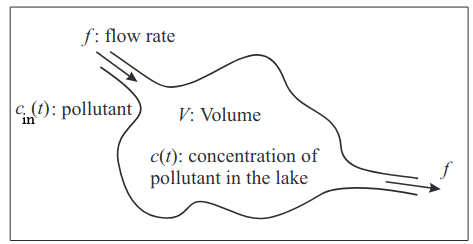
\includegraphics[height=4cm]{img/lake/lake_model_diagram.png}
    \caption{The constant flow lake model.}
    \label{fig:my_label}
\end{figure}

Therefore the mass of pollutant entering the lake at any time is:
\[
M_{in}(t) = f(t)c_{in}(t)
\tag{2}
\]
The concentration anywhere in the lake is $M(t)/V$ and the water flows out at ($m^3/day$) at $f(t)$. Therefore at any time, the mass leaving the lake is:
\[
M_{out}(t) = \frac{f(t)}{V}M(t) = f(t)c_{in}(t)
\tag{3}
\]
Formulating the model and using Eq. (1)-(3):
\begin{gather*}
    \frac{dM}{dt} = M_{in} - M_out  \Rightarrow \\
    V\cdot c'(t) = f(t)\cdot c_in(t) -  f(t)c_{in}(t) \Rightarrow \\
    c'(t)  = \frac{f(t)}{V}c_{in} - \frac{f(t)}{V}c(t) \Rightarrow  \\
    c'(t) = \frac{f(t)}{V}\big(c_{in} - c(t) \big) \label{eq:ode_lake_as_in_cooling} \tag{4}
\end{gather*}

The flow $f(t)$ may or may not be constant. For instance, it may vary depending on the season, with the maximum reached at the peak of rainy season and the minimum in summer. $c(t)$ may also vary. However, the case where both $f(t)$ and $c(t)$ are constant leads to a simpler solution.

\begin{enumerate}
    \item (\textit{Constant flow with constant concentration}) If $f(t)$ and $c_{in}(t)$ respectively are constant,  then the concentration equation Eq. (4) can be solved exactly the same way as Newton's law of cooling equation (\eqref{eq:newtons_law_cooling}). According to \eqref{eq:newtons_law_cooling_sol}, the solution is:
    \[
        c(t) = c_{in} + e^{-\frac{f}{v}t} (c(0) - c_{in})
    \]
    , where $c(0)$ is the initial condition, i.e. the concentration of pollutant in the lake at $t=0$.
    
    \item (\textit{Variable flow, variable concentration}) In this case $f(t)$ is variable and periodical depending on the day of the year, e.g. 
    \[
        f(t) = f_0\left(1 + \epsilon\sin\left(\frac{2\pi}{T}t\right)\right)
    \]
    , $T$ is the period, e.g. $365$ days, $f_0$ is the mean annual flow and $\epsilon$ is the normalised flow amplitude, therefore $\left| \epsilon \right| \leq 1$. This ensures that $f(t) \geq 0$. $c(t)$ may also be variable and depending on the day of the year in a similar manner. Then \eqref{eq:ode_sep_dy} is written as:
    \begin{gather*}
        c'(t) = \frac{f(t)}{V}\left(c_{in}(t) - c(t)\right) = \frac{f_0\left(1 + \epsilon\sin\left(\frac{2\pi}{T}t\right)\right)}{V}\left(c_{in}(t) - c(t)\right) \Rightarrow \\
        c'(t) +\frac{f(t)}{V}c(t) = \frac{f(t)c_{in}(t)}{V}
        \tag{5}
    \end{gather*}
    This is a non-homogeneous first order DE (\eqref{eq:nonhomo_first_order}) and we know it  can be solved by the integrating factor method. Let's be pedantic and solve it step-by-step.
    \begin{gather*}
        c'(t) +\frac{f(t)}{V}c(t) = \frac{f(t)c_{in}(t)}{V}
    \end{gather*}
    Multiplying both sides by $\exp\left(\int \frac{f(t)}{V}\, dt\right)$:
    \begin{gather*}
        c'(t)\underbrace{\exp\left(\int \frac{f(t)}{V}\, dt\right)}_{u(t)} + c(t)\underbrace{\exp \left(\int \frac{f(t)}{V}\, dt\right)'}_{u'(t)} = \frac{f(t)c_{in}(t)}{V} \underbrace{\exp\left(\int \frac{f(t)}{V}\, dt\right)}_{u(t)}
    \end{gather*}
    \begin{gather*}
        \big( c(t)u(t) \big)' =  \frac{f(t)c_{in}(t)}{V} u(t)
    \end{gather*}
    Now, since we know the initial condition $c(t_0) = c_0$ and we want to find $c(t)$, we integrate from $t_0$ to $t$ and replace dummy variable $t$ with dummy variable $s$ in the integral term:
    \[
        c(t)u(t) - c(t_0)u(t_0) = \int_{t_0}^t \frac{f(s)c_{in}(s)}{V} u(s) \, ds
    \]
    \[
        c(t) = \frac{1}{u(t)}
        \left\{  \int_{t_0}^t  \frac{f(s)c_{in}(s)}{V} u(s) \, ds + c(t_0)u(t_0) \right\}, \quad u(s) = \exp \left(\int\frac{f(s)}{V}\, ds\right)
        \label{eq:ode_lake_general_sol}
        \tag{6}
    \]
\end{enumerate}
\begin{exmp}
The average summer flow into an out of a lake is $4\cdot 10^6\; m^3/\textup{month}$. The volume of that lake is constant and equal to $28\cdot 10^6 \; m^3$. When the measurements start at $t=0$, the initial concentration of pollutant is $c(0) = 10^7 \; \textup{parts}/m^3$. If there is no more pollution since the measurements have started, how long will it take for the lake pollution level to drop to $5\%$ of its initial level?
\end{exmp}
\begin{soln}
When $f(t)$ and $c_{in}(t)$ are constant, we have derived that the pollutant concentration is given by:
 \[
    c(t) = c_{in} + e^{-\frac{f}{v}t} (c(0) - c_{in})
\]
Plugging in the data:
\[
    c(t) = 0 + e^{-t/7} (c_0 - 0) = c_0e^{-t/7}
\]
We want a $t_1$ s.t. $c(t_1) = 0.05c_0 \Rightarrow  c_0e^{-t_1/7} = 0.05c_0 \Rightarrow t_1 = -7\ln(0.05) = 20.97 \; \textup{months}$.
\end{soln}

\begin{exmp}
Consider the same lake ($V = 28\cdot 10^6\; m^3$). Assume that $c_0$ is known but not necessarily zero. Plot the pollution mass over time $t\in [0,100]$ in the lake $c(t)$ for the following cases:
\begin{enumerate}
    \item $f = 4\cdot 10^6$, $c_{in}(t) =3\cdot 10^6$
    \item $f = 4\cdot 10^6$, $c_{in}(t) = 10^7(1+\cos(2\pi t))$
    \item $f(t) = 10^6(1+6\sin(2\pi t))$, $c_{in} = 3\cdot 10^6$
    \item $f(t) = 10^6(1+6\sin(2\pi t))$, $c_{in} = 10^7(1+\cos(2\pi t))$
\end{enumerate}
Consider the initial conditions for the concentration in the lake $c_0 \in \{1,7/3,11/3,5\}\times 10^6$.
\end{exmp}

\begin{soln}
\begin{enumerate}
    \item Since both $f(t)$ and $c_{in}(t)$ are constant, the solution is given by Newton's law of cooling:
    \begin{align*}
         c(t) &= c_{in} +\exp\left(-ft/V\right) - c_{in}) \\
         &= 3\cdot 10^6 + \exp\left(- t/7\right)\cdot (c_0 - 3\cdot 10^6)
    \end{align*}

    \item We use Eq. (6) to find the general solution:
    \[
        u(s) = \exp \left(\int\frac{f(s)}{V}\, ds\right) = \exp \left(\int  \frac{1}{7}\, ds\right) = \exp\left(\frac{s}{7}\right)
    \]
    (We drop the constant). The general solution is then given by:
    \begin{align*}
        c(t) &= \frac{1}{u(t)}
        \left\{  \int_{t_0}^t  \frac{f(s)c_{in}(s)}{V} u(s) \, ds + c(t_0)u(t_0) \right\}, \quad u(s) = \exp \left(\int\frac{f(s)}{V}\, ds\right) \\
         &= \exp\left(-\frac{t}{7}\right) \left\{
         \int_{t_0}^t \frac{4\cdot 10^6}{28\cdot10^6} \cdot 10^7\big(1+\cos(2\pi s)\big) \cdot \exp\left(\frac{s}{7} \right) \, ds
         + c_0u(t_0) \right\}, \quad t_0 = 0 \\
         &= \exp\left(-\frac{t}{7} \right) \left\{\frac{1}{2+392\pi^2}2\cdot10^7 \left(
            -2 -196\pi^2 + 
            e^{t/7}\left(
                1 + 196\pi^2 + \cos(2 \pi t) + 14 \pi \sin(2\pi t)
            \right)
         \right) + c_0u(0)
         \right\}
    \end{align*}
    
    \item The general solution is given by the same formula. First. we find an integrating factor and then substitute it in the formula for $c(t)$.
    \[
        u(s) = \exp\left(\int \frac{f(s)}{V}\, ds \right) = \exp\left( \frac{1}{28} \int (1+6\sin(2\pi s))\, ds \right) = \exp \left(\frac{1}{28} \left(s - \frac{3\cos(2\pi s)}{\pi} \right)
        \right)
    \]
    \begin{align*}
        \therefore c(t) &= \frac{1}{u(t)}
        \left\{  \int_0^t  \frac{f(s)c_{in}(s)}{V} u(s) \, ds + c(0)u(0) \right\} \\
        &=   \exp \left(\frac{1}{28} \left( \frac{3\cos(2\pi s)}{\pi} - s \right)
        \right)
        \left\{  \int_0^t  \frac{ 10^6(1+6\sin(2\pi s)) \cdot 30\cdot 10^6}{28\cdot 10^6} \exp \left(\frac{1}{28} \left(s - \frac{3\cos(2\pi s)}{\pi} \right)
        \right) \, ds + c(0)u(0) \right\}
    \end{align*}
    Such integrals can be extremely tedious or impossible to compute analytically, so it's preferred to solve this ODE in a software package, such as  Matlab/Octave or Python. ODE solvers in Matlab (\texttt{ode23}) and Python (\texttt{scipy.integrate.odeint}) take the same arguments so here are  these are a few things to remember before invoking them:
    \begin{enumerate}
        \item The ODE to solve must be in the form $y' = a(x)y + b(x)$ ($x$ is the free variable like $t$).
        \item The solver works recursively by computing $y'$ for different values of $t, y$.
        \item Therefore the solver takes as arguments a function $f$ that describes our ODE (the function itself, not its return $f(t,x)$!), the sampled free variable $x$, and the initial condtion $y_0 = y(t_0)$. It returns the particular solution for the said initial condition.
    \end{enumerate}
    The Matlab solution given the data in this question is listed in \ref{app:code_lake_pollution}.
    
    \item Similarly to part (c), to plot the particular solutions $c(t)$ for various $c(0)$ and for the data $f(t) = 10^6(1+6\sin(2\pi t))$, $c_{in} = 10^7(1+\cos(2\pi t))$ can be plotted in Matlab by the \texttt{lake} function in \ref{app:code_lake_pollution}.
    % see also  https://jmahaffy.sdsu.edu/courses/f15/math337/beamer/matlab/matlab_linear.pdf
\end{enumerate}
In the end, we obtain the following four figures for the concentrations given the data in each part.

\begin{multicols}{2}
\begin{figure}[H]
    \centering
    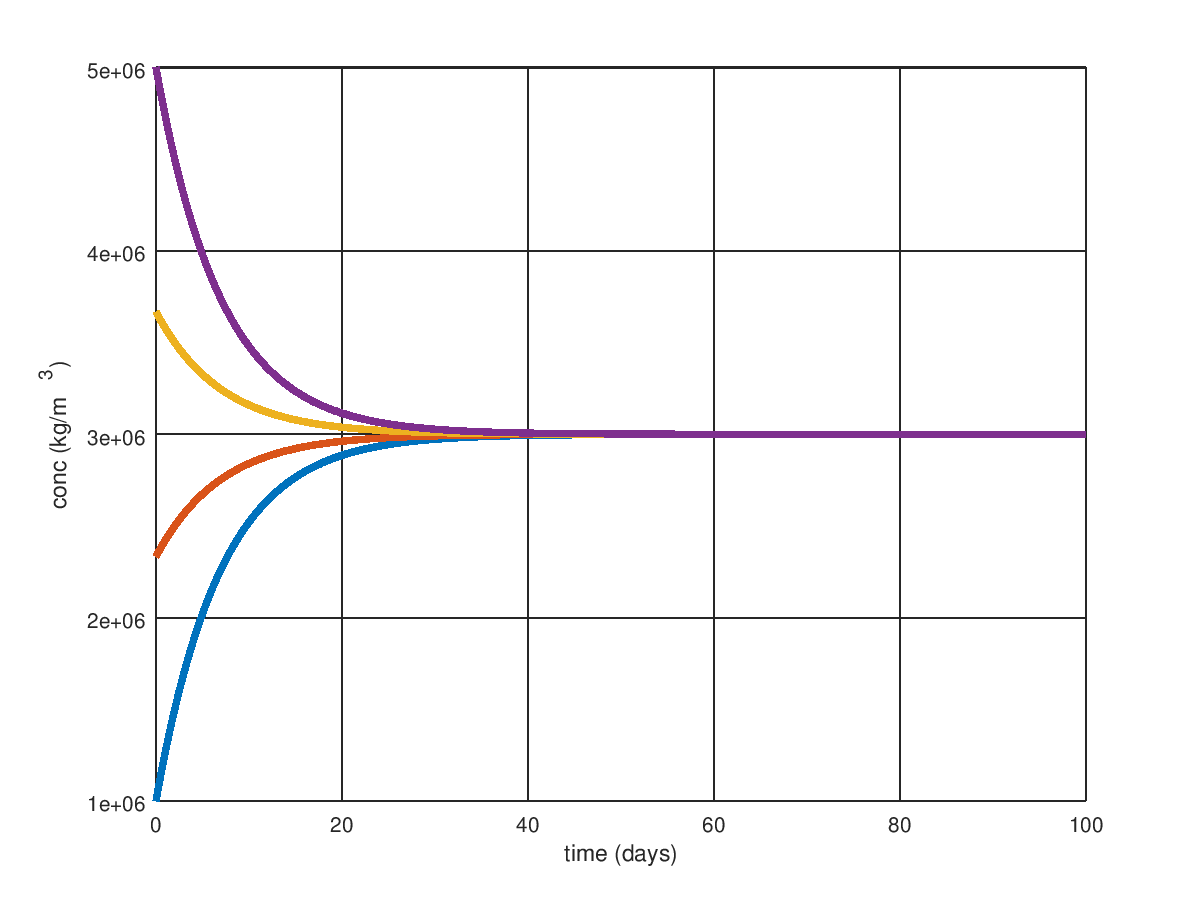
\includegraphics[height=4.5cm]{img/lake/c_const_f_const.png}
    \caption{Lake pollution solution for constant pollution and flow.}
    \label{fig:my_label}
\end{figure}

\columnbreak
\begin{figure}[H]
    \centering
    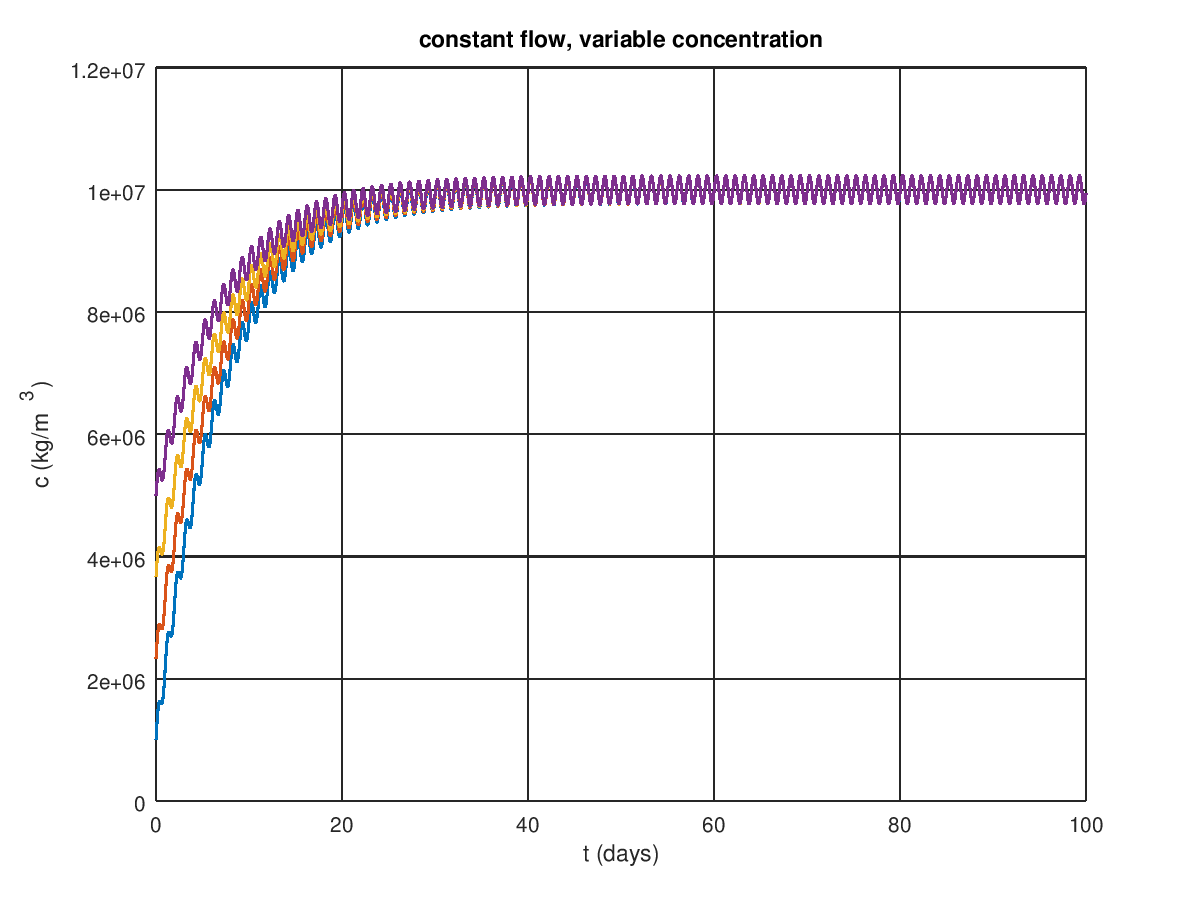
\includegraphics[height=4.5cm]{img/lake/c_var_f_const.png}
    \caption{Lake pollution solution for constant pollution and variable flow.}
    \label{fig:my_label}
\end{figure}
\end{multicols}

\begin{multicols}{2}
\begin{figure}[H]
    \centering
    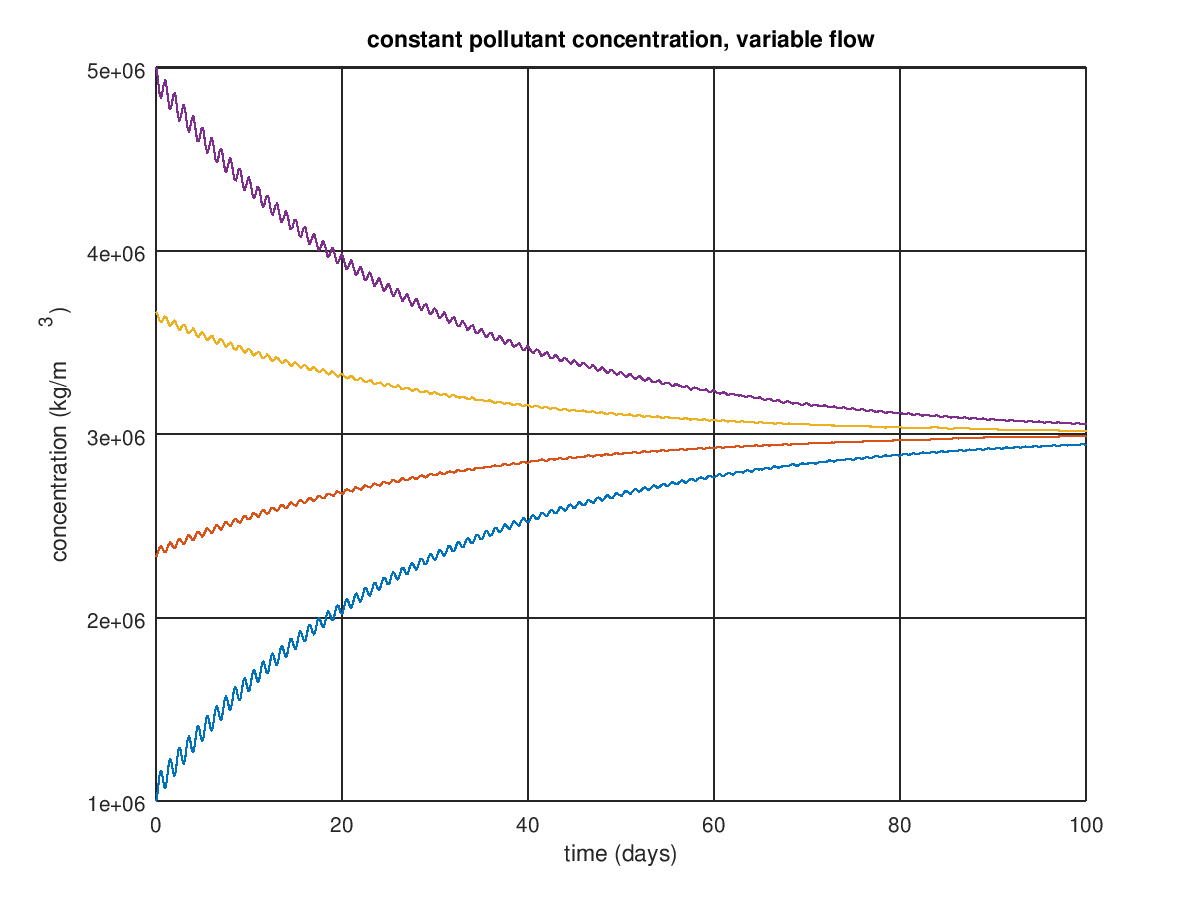
\includegraphics[height=4.5cm]{img/lake/c_const_f_var.png}
    \caption{Lake pollution solution for constant pollution and variable flow.}
    \label{fig:my_label}
\end{figure}

\columnbreak
\begin{figure}[H]
    \centering
    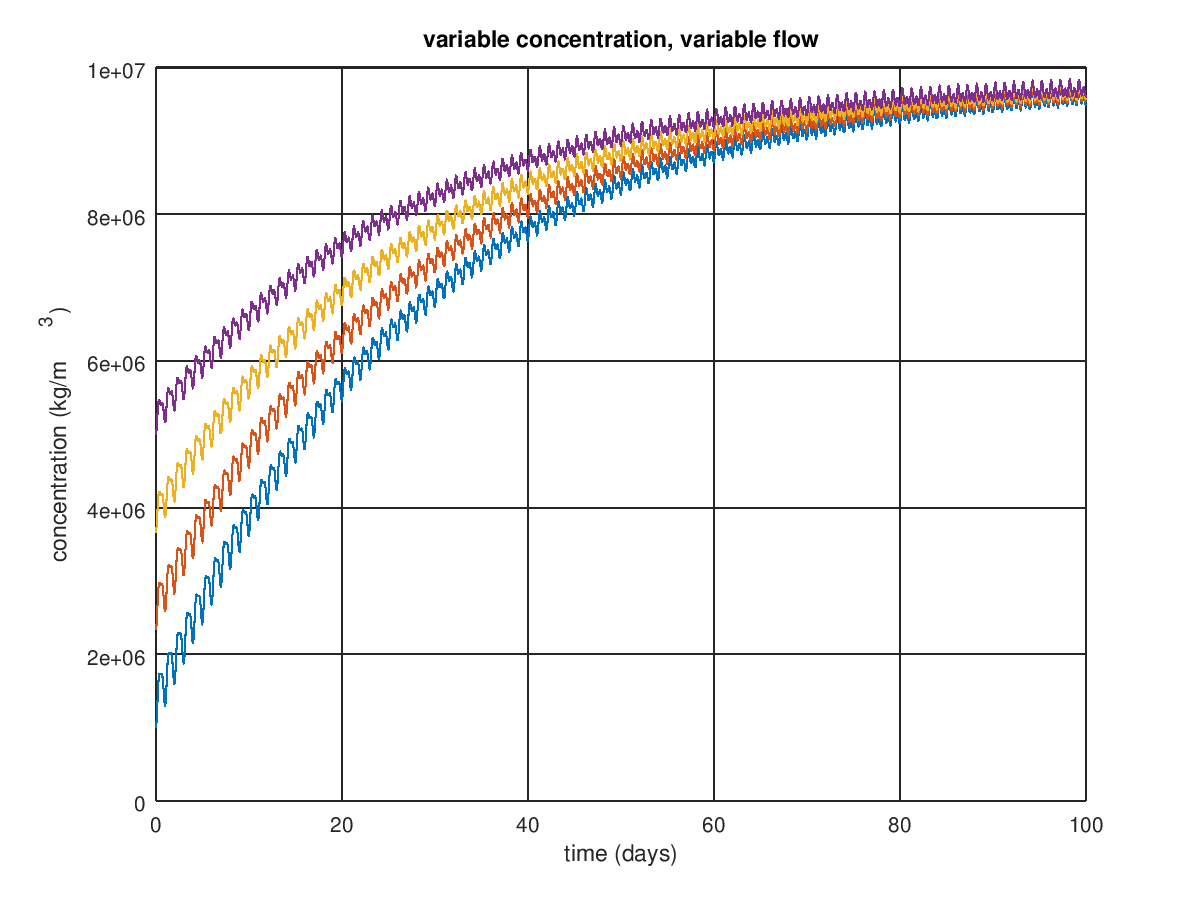
\includegraphics[height=4.5cm]{img/lake/c_var_f_var.png}
    \caption{Lake pollution solution for variable pollution and flow.}
    \label{fig:my_figure}
\end{figure}
\end{multicols}
When $c_{in}$ is constant, $c(t)$ converges to $c_{in}$
\end{soln}






%\subsection{Application 3: Pursuit Curves}
%\TODO

\subsection{Directional Fields}

A \emphasis{directional field} (a.k.a. slope field) a set of tiny segments in the 2D space, each of which approximates the slope of a function at each point. The segment are draw in a sampled region of the 2D space. Slope fields are used to  roughly illustrate the solution of an ODE of the form $\tfrac{dy}{dx} = f(x,y)$ by drawing $\tfrac{dy}{dx}$ without explicitly knowing them. If we connect such segments together so that they're all tangent to the same curve, we can graphically approximate a particular solution to $\tfrac{dy}{dx} = f(x,y)$. 

This sounds vague so it's best to draw a slope field of an actual ODE. 

\begin{exmp}
Sketch the flow field of the solution to:
\[
\frac{dy}{dx} = y-x
\]
Plot it over $[0, 5] \times [0, 6]$.
\end{exmp}
\begin{soln}
The equation is already in a form where $\tfrac{dy}{dx}$ can be evaluated. Therefore we can iterate over all $x$'s and $y$'s with a certain step, e.g. 1, and compute $\tfrac{dy}{dx}$. Before sketching the actual field, let's think that the given ODE tells us about the derivative -- the larger the absolute different between $x$ and $y$, the steeper the magnitude. Along the line $y=x$, the line will be flat. Above $y=x$, the slope is positive and below it negative.

The field is drawn by a slightly modified version of \href{thttps://github.com/tamaskis/slope_field-MATLAB/blob/main/slope_field.m script}{tamaskis's script} function which is supported by Octave too. The source code is found in \ref{app:code_slope_field}. Two solutions are roughly sketched in magenta in Fig. \ref{fig:flow_field_of_y_x}.

\begin{figure}[H]
    \centering
    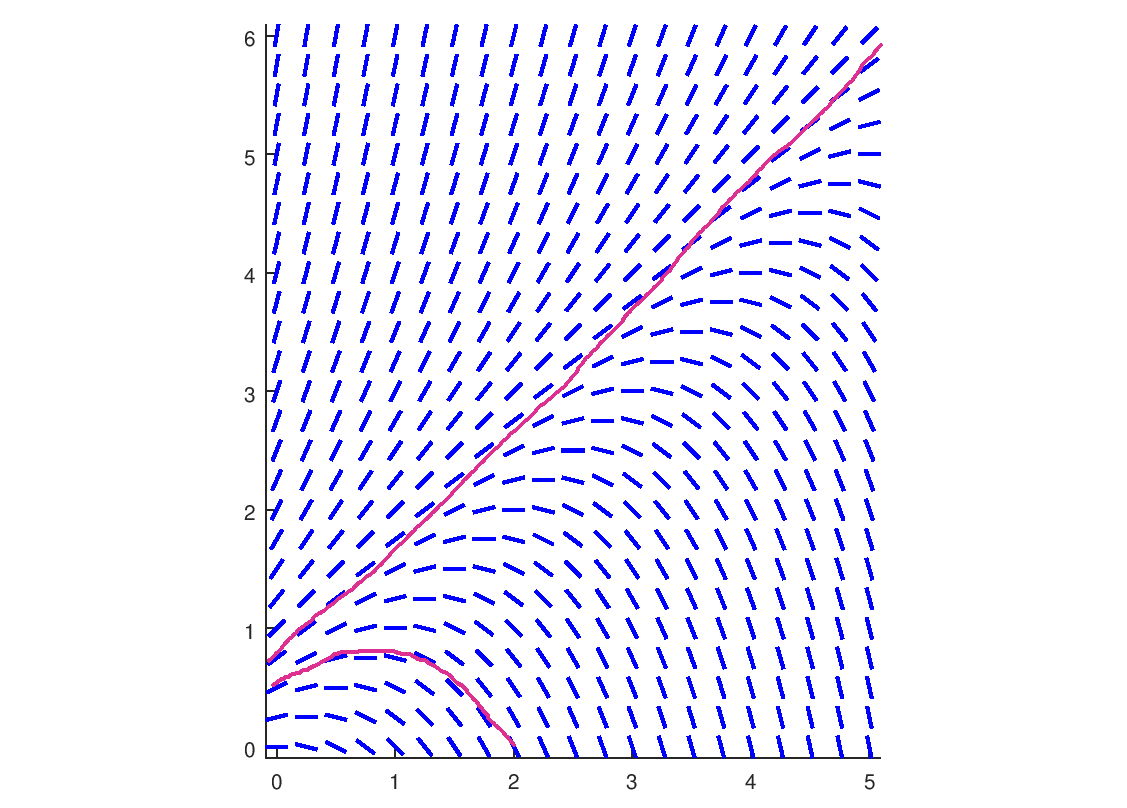
\includegraphics[height=4.5cm]{img/flow_fields/slope_field_of_y-x.png}
    \caption{Slope field of the solutions to $y' = y - x$ with two solutions roughly drawn.}
    \label{fig:flow_field_of_y_x}
\end{figure}
\end{soln}

% ref https://www3.nd.edu/~apilking/Math10560/Lectures/18.%20Direction%20Fields%20Euler%27s%20Method.pdf
% https://www.youtube.com/watch?v=D3V5FmAUrpE
% beautiful fields:  https://ximera.osu.edu/ode/main/directionFields/directionFields
% https://www.maplesoft.com/applications/view.aspx?SID=4702&view=html
% https://www.youtube.com/watch?v=MI2xCwBekX4


\subsection{Numerical Methods: Euler's Method}

Often it's impossible to analytically solve a 1st order ODE with the techniques described. In this case it needs to be solved (approximated) numerically.
% nicer diagram: https://www.freecodecamp.org/news/eulers-method-explained-with-examples/
\begin{figure}[H]
    \centering
    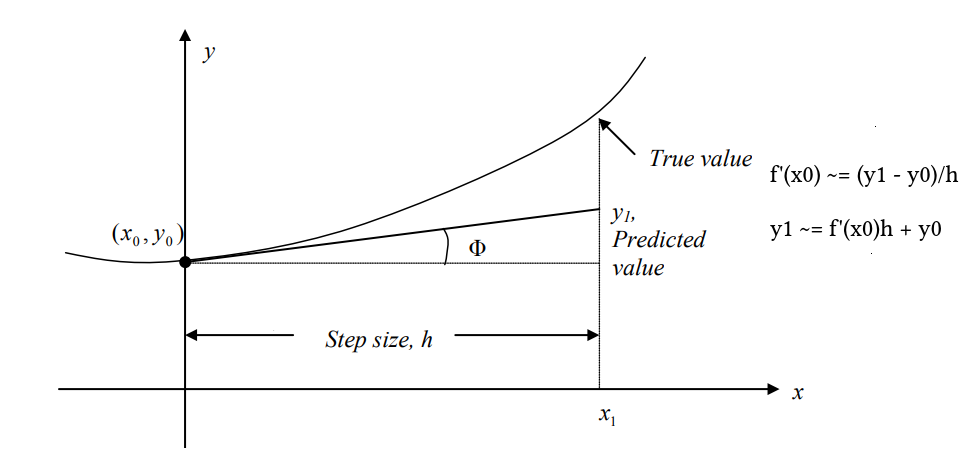
\includegraphics[height=5cm]{img/euler/eulers_method_sketch.png}
    \caption{Euler's method approximates the solution by a continuous set of segments tangent to the original curve.}
    \label{fig:eulers_method_idea}
\end{figure}

Euler's method estimates a particular solution curve $y_p(x)$ to the ODE $y'=f(x,y)$ using some finite points $y_{p,i}$.\marginnote{Euler's method works for both linear and non-linear ODEs.}It considers the curve as a connected set as some infinitesimal straight segments, each segment being defined by two points $(x_{i-1}, y_{p,i-1})$, $(x_{i}, y_{p,i})$. Point $i$ is estimated given point $i-1$. As each segment is straight, point $i$ is estimated via the derivative at $i-1$. Referring to Fig. \ref{fig:eulers_method_idea}, one can estimate $y_1$ given $y_0$ as:
\begin{gather*}
    y'_{0} = \frac{y_1-y_0}{x-x_0} = \frac{y_1-y_0}{h} \Rightarrow \\
    y_1  = y_{0} + h\, y'_0 \Rightarrow \\
    y_1 = y_0 + h\, f(x_0,y_0)
\end{gather*}
The last equation comes from the fact that we are trying to solve the 1st order ODE  $y'=f(x,y)$. $h$ is the step size -- a small fraction of the range of the $x$ domain where we want to solve the equation on.  Euler's method works iteratively, starting from $y_0$ to $y_1$ to $y_n$.
\begin{corollary}[Euler's method (1st order ODEs)]
A particular solution $y_p$ to a 1st order ODE
\[
\frac{dy}{dx} = f(x,y)
\]
can iteratively be approximated in a domain $[x_{min}, x_{max}]$ by Euler's method as:
\begin{equation}
        y_{p,i} = y_{p,i-1} + h\, f(x_{i-1},y_{i-1})
\end{equation}
, where $h$ is the step size $h:=\tfrac{x_{max} - x_{min}}{N}$. Furthermore $y_{p,0} = y(t_0)$ is known from the initial condition.
\end{corollary}

Euler's method can easily be coded e.g. in Matlab (\ref{app:code_eulers_method}).

\begin{exmp}
% see https://www-thphys.physics.ox.ac.uk/people/FrancescoHautmann/Cp4/sl_ode_11_2.pdf
Solve the following ODE using Euler's method for $x\in [0.4,0.8]$ for step sizes $h=0.02,0.01$. Solve it analytically and compare the numerical solution to the analytical one. 
\[
\frac{dy}{dx} = (-4x+y)^2, \quad -4x + y > 2, \quad y(0.4) = 4
\]
\end{exmp}
\begin{soln}
\marginnote{Remember $y$ is a function of $x$!}Let's solve it analytically first. It can be solved by change of variables. Let
\begin{gather*}
    z := -4x + y \Rightarrow \\
    \frac{dz}{dx} = \frac{d(-4x + y)}{dx} = -4 + \frac{dy}{dx} \Rightarrow \\
    \frac{dz}{dx} = -4 + z^2
\end{gather*}
This can be re-arranged as a separable equation ($M(x)dx = N(z)dz$ -- see \eqref{eq:ode_separable}):
\[
4dx = \frac{dz}{(z-2)(z+2)} = \frac{dz}{z-2} -  \frac{dz}{z+2}  
\]
Both sides can now be integrated and their integrals can be computed:
\begin{gather*}
    4x = \ln\left|z-2 \right| - \ln\left|z+2 \right|\Rightarrow \\
    4x + C = \ln \left(\frac{\left|z-2 \right|}{\left|z+2 \right|} \right) = \ln \left(\frac{z-2}{z+2} \right)
\end{gather*}
Solve for $z$, hence for $y$:
\begin{gather*}
    e^{4x} = \frac{z-2}{z+2} \Rightarrow \\
    z = 2 \frac{1+Ce^{4x}}{1-Ce^{4x}} =   2 \frac{1-Ce^{4x} + 2Ce^{4x}}{1-Ce^{4x}} = \frac{4}{1-Ce^{4x}} -2
\end{gather*}
Substitute back for $y$ from $z = y-4x$:
\begin{gather*}
    y = \frac{4}{1-Ce^{4x}} + 4x - 2
    \tag{1}
\end{gather*}
Plugging in the initial condition $x,y=0,4$, we obtain $C\approx 0.0183 $. This is the analytical (``true'') solution.

The numerical approximation is computed using the code in \ref{app:code_eulers_method}, e.g. from the following lines. Increasing the step size by 10 significantly reduces the error.
\begin{verbatim}
f = @(x,y) ((-4*x+y)^2)
C = 0.0183;
h = 0.01;
%       (f, [xmin, xmax], f(xmin), h)
[x,y] = myeuler(f, [0.4,0.8], 4, h);
\end{verbatim}
Plotting the analytical solution, approximations for $h=0.02$ and $h=0.01$ we observe the error is significantly reduced by halving the step:
\begin{figure}[H]
    \centering
    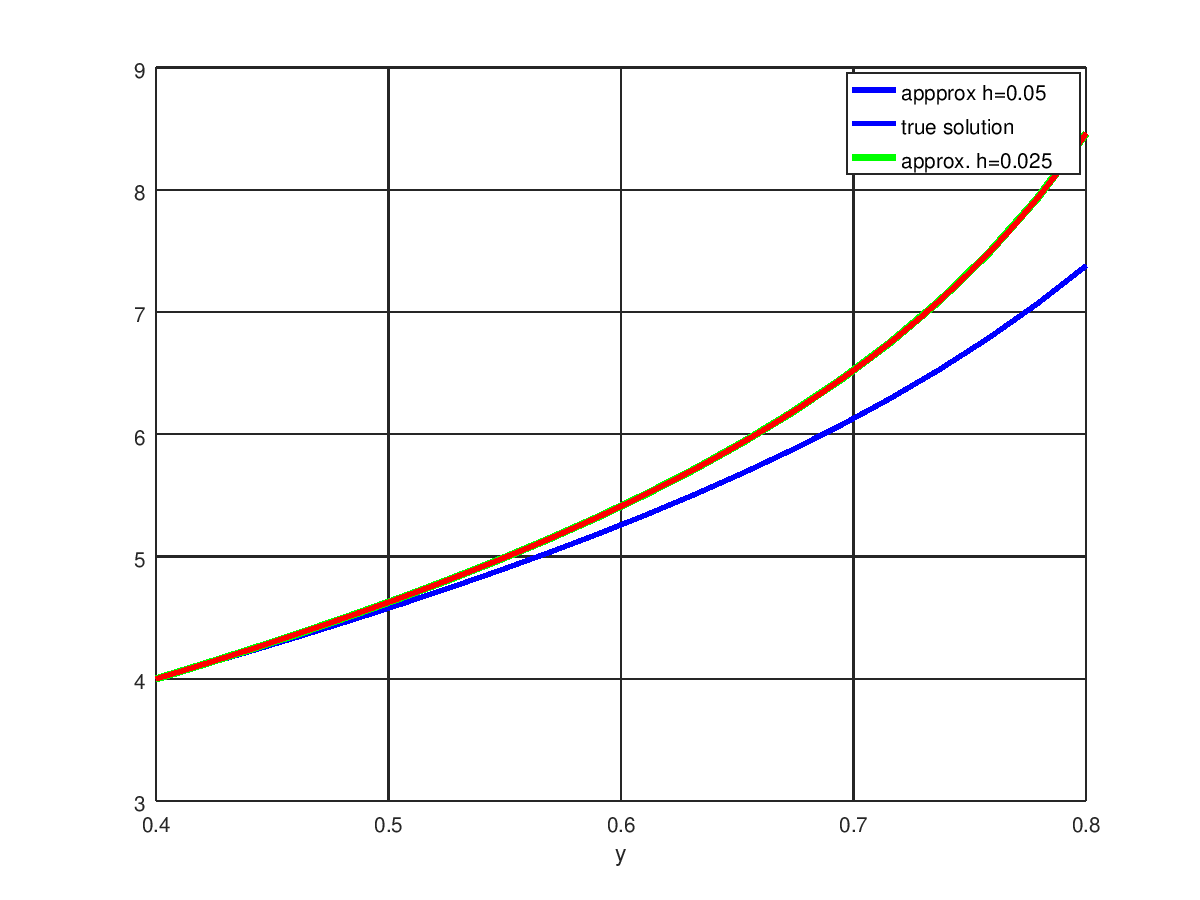
\includegraphics[height=5.5cm]{img/euler/example_euler_anal_approx.png}
    \caption{The analytical solution to $y' = (-4x+y)^2$ vs two approximations.}
\end{figure}
\end{soln}

% error:
% https://ocw.mit.edu/courses/aeronautics-and-astronautics/16-90-computational-methods-in-aerospace-engineering-spring-2014/numerical-integration-of-ordinary-differential-equations/order-of-accuracy/1690r-local-truncation-error/
% https://ximera.osu.edu/laode/textbook/numericalSolutionsOfODEs/errorBoundsForEulersMethod
% https://math.libretexts.org/Courses/Monroe_Community_College/MTH_225_Differential_Equations/3%3A_Numerical_Methods/3.1%3A_Euler%27s_Method
% https://personal.math.ubc.ca/~israel/m215/euler2/euler2.html
% https://www.math.rutgers.edu/docman-lister/math-main/academics/course-materials/252/1543-euler-pdf/file
% https://web.mit.edu/10.001/Web/Course_Notes/Differential_Equations_Notes/node5.html
% https://www.colorado.edu/amath/sites/default/files/attached-files/rk_derivation_0.pdf
% https://web.mit.edu/10.001/Web/Course_Notes/Differential_Equations_Notes/node5.html
% https://mathforcollege.com/nm/mws/gen/08ode/mws_gen_ode_txt_runge2nd.pdf
% http://www.math.iit.edu/~fass/478578_Chapter_3.pdf
% http://sites.iiserpune.ac.in/~pgoel/RungeKutta.pdf
% https://www.youtube.com/watch?v=hhgG8KL_pCk
% https://www.youtube.com/watch?v=2vslKRPlgo0
% https://www.youtube.com/watch?v=2vslKRPlgo0
% https://books.google.gr/books?id=FYs1-SGPbrQC&pg=PA461&dq=runge-kutta&hl=en#v=onepage&q=runge-kutta&f=false
% https://web.mit.edu/10.001/Web/Course_Notes/Differential_Equations_Notes/node5.html
%




\subsection{Numerical Methods: Runge-Kutta Method}

Euler's method is simple to implement but may be inaccurate, as it assumes that the slope is constant in interval $[x_n, x_{n+1}]$ and only takes into account the slope at $x_n$.

Runge-Kutta (RK) methods are a family of methods to solve an ODE $\tfrac{dy}{dx} = f(x,y)$ given an initial value $y(t_0)=y_0$. RK methods are
\begin{itemize}
    \item iterative (when we know $y_n$, we compute $y_{n+1}$ as $y_{n+1} = y_n + \textup{increment}$)
    \item more accurate than Euler's  since they compute the weighted average of the slopes at interval $[x_n, x_{n+1}]$,
    \item efficient as they do not rely on the derivatives $f_(x,y)$,
    \item more expensive than Euler's explicit method.
\end{itemize}
% ref https://ocw.snu.ac.kr/sites/default/files/NOTE/Lecture%2010_0.pdf
They rely on the Taylor series expansion of $f(x,y)$. RK2 require two evaluations of $f(x,y)$ within each sub-interval $[x_n, x_{n+1}]$, RK4 require four, etc. We shall derive the 2nd order RK method (RK2) and then formulate the 4th order one. In RK2, the increment is a weighted average of two quantities $K_1, K_2$, i.e.
\[
y_{n+1} = y_n + \alpha K_1 + \beta K_2
\]
, where $\alpha$ and $\beta$ are constants. $\alpha, \beta, K_1, K_2$ are chosen such that they satisfy a certain set of constraints.
\begin{definition}[Runge-Kutta 2]
Given the initial value problem
\[
\frac{dy}{dx} = f(x,y)
\]
, the general form of 2nd order Runge-Kutta methods that solve it is:
\begin{equation}
    y_{n+1} = y_n + \textup{a} K_1 + b K_2
\end{equation}
, where
\begin{equation}
    \left \{
        \begin{array}{l}
             K_1 = h f(x_n, y_n)  \\
             K_2 = h f(x_n + \alpha h, y_n + \beta K_1)
        \end{array}
    \right.
\end{equation}
$h$ is the step size.
\end{definition}
Before the RK2 method is applied, $\alpha, \beta, \textup{a}, b$ are chosen by the user. We will prove that certain constraints must hold for them, particularly:
\begin{equation}
    \left \{
        \begin{array}{l}
            \textup{a} + b = 1 \\
            b \beta = \frac{1}{2} \\
            \alpha b = \frac{1}{2}
        \end{array}
    \right.
\end{equation}
\begin{proof}
To determine the constants, we first expand (by Taylor series) $y_{n+1} $ (denoting $y_n = y(x_n), y_{n+1} = y(x_{n+1})$) at a neighbourhood around $x_{n}$ up to the $h^2$ term:
% ref https://web.mit.edu/10.001/Web/Course_Notes/Differential_Equations_Notes/node5.html
\[
    y_{n+1} = y_n + h\left. \frac{dy}{dx} \right|_{x_n} + \frac{h^2}{2}\left.\frac{d^2y}{dx^2}\right|_{x_n} + \mathcal{O}(h^3)
    \tag{1}
\]
However, since we're trying to solve the problem $\tfrac{dy}{dx} = f(x,y)$, Eq. (1) can be rewritten as:
\[
    y_{n+1} = y_n + hf(x_n,y_n)+ \frac{h^2}{2}f'(x_n,y_n) + \mathcal{O}(h^3)
    \tag{2}
\]
However, from the total derivative/total differential formula, we know for $f'(x_n,y_n)$:
\begin{align*}
    f'(x_n,y_n) &= \frac{\partial f(x_n,y_n)}{\partial x}\frac{dx}{dx} + \frac{\partial f(x_n,y_n)}{\partial y} \frac{dy}{dx} \\
    &= \frac{\partial f(x_n,y_n)}{\partial x} + \frac{\partial f(x_n,y_n)}{\partial y} f(x_n,y_n)
\end{align*}
Therefore Eq. (2) is rewritten in terms of the partial derivatives and $f(x,y)$ as:
\[
y_{n+1} = y_n + hf(x_n,y_n)+ \frac{h^2}{2}
\left[ \frac{\partial f(x_n,y_n)}{\partial x} + \frac{\partial f(x_n,y_n)}{\partial y} f(x_n,y_n)  \right]
\tag{3}
\]
It turns out that we can also write the update step $y_{n+1} = y_n + \textup{a}K_1 + b K_2$ as a polynomial of $h$, whose each coefficient depends on $f$ and its partial derivatives. First, expand $K_2 = f(x_n + \alpha h, y_n + \beta K_1)$ by multivariate Taylor series:
\begin{align*}
    K_2 &= h f(x_n + \alpha h, y_n + \beta K_1) \\
    &= h \left[ f(x_n, y_n) + \frac{\partial f(x_n, y_n)}{\partial x} \alpha h + \frac{\partial f(x_n, y_n)}{\partial y} \beta h f(x_n, y_n) \right]
\end{align*}
Then the update equation is:
\begin{align*}
    y_{+1} &= y_n + \textup{a} h f(x_n, y_n) + b h \left[ f(x_n, y_n) + \frac{\partial f(x_n, y_n)}{\partial x} \alpha h + \frac{\partial f(x_n, y_n)}{\partial y} \beta h f(x_n, y_n) \right] \\
    &= y_n + h(\textup{a} + b) f(x_n, y_n) + \frac{\partial f(x_n, y_n)}{\partial x} \alpha b h^2 + \frac{\partial f(x_n, y_n)}{\partial y} b \beta f(x_n, y_n) h^2 + \mathcal{O}(h^3)
    \tag{4}
\end{align*}
By matching terms in Eq. (3), (4), we can find the constants $\textup{a}, b, \alpha, \beta$. Comparing each polynomial coefficients and each derivative term we obtain:
\[
    \left \{
        \begin{array}{l}
            \textup{a} + b = 1 \\
            b \beta = \frac{1}{2} \\
            \alpha b = \frac{1}{2}
        \end{array}
    \right.
\]
These equations summarise the possible choices of constants $\textup{a}, b, \alpha, \beta$ that satisfy RK2.
\end{proof}
Therefore there are infinitely many choices for $\textup{a}, b, \alpha, \beta$. A popular and fairly accurate RK2 method is Heun's, which selects $\textup{a} = 1/2, b=1/2, \alpha = 1, \beta = 1$. Heun's method averages the two slopes at the ends $x_n, x_{n+1}$ of each sub-interval $[x_n, x_{n+1}]$. Then the RK2 equations become:
\begin{align*}
    y_{n+1} &= y_n + \frac{K_1}{2} + \frac{K_2}{2} \\
    K_1 &= h(x_n,y_n) \\
    K_2 &= h\, f(x_n + h, y_n + K_1)
\end{align*}
Visually, Heun's RK2 method is illustrated below. Note that we don't take the second slope at point $(x_n+h, y_n)$, which is on the graph, but at $(x_n+h, y_n + K_1)$.
\begin{figure}[H]
    \centering
    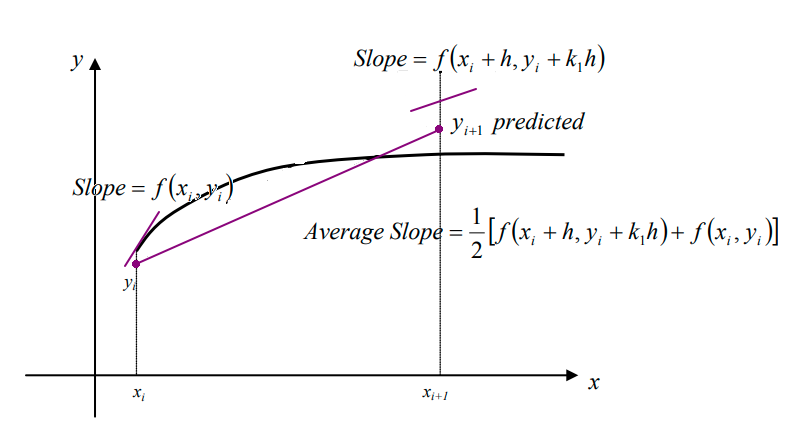
\includegraphics[height=4cm]{img/rk/diagram_heun.png}
    \caption{The two slopes that Heun's (a RK2) method takes into account.}
\end{figure}


Runge-Kutta 4th order (RK4) method can be proven in the same fashion as RK2 but its proof is omitted here. It can be stated as follows.
\begin{definition}[Runge-Kutta 4]
% ref https://books.google.gr/books?id=FYs1-SGPbrQC&pg=PA461&dq=runge-kutta&hl=en#v=onepage&q=runge-kutta&f=false
The general form of the RK4 method is
\begin{align}
    k_1 &= hf(x_n,y_n) \\
    k_2 &= hf(x_n + \alpha_2h, y_n + \beta_2 k_1) \\
    k_3 &= hf(x_n + \alpha_3h, y_n + \beta_3 k_1 + \beta_3' k_2) \\
    k_4 &= hf(x_n + \alpha_4h, y_n + \beta_4 k_1 + \beta_4' k_2 + \beta_4'' k_3) \\
    y_{n+1} &= y_n + a_1\textup{a}_1 k_1 + \textup{a}_2 d_2 + \textup{a}_3 k_3 + \textup{a}_4 k_4
\end{align}
\end{definition}
A popular RK4 method uses the values of $\alpha_2=1/2, \beta_2 = 1/2, b_3 = 0, b_3' = 1/2, a_4 = 1, b_4 = b_4' = 0, b_4''=1, \textup{a}_1 = 1/6, \textup{a}_2 = \textup{a}_3 = 2/6, \textup{a}_4 = 1/6$. In this case, the RK4 formulas as follows. Note that to find the new estimate of the solution ($y_{n+1}$), we increment $y_n$ by the weighted sum of four slopes $k_1,k_2,k_3,k_4$.
\begin{align}
    k_1 &= hf(x_n,y_n) \label{eq:rk4_1_1} \\
    k_2 &= hf(x_n + \frac{h}{2}, y_n + \frac{k_1}{2}) \\
    k_3 &= hf(x_n + \frac{h}{2}, y_n + \frac{k_2}{2}) \\
    k_4 &= hf(x_n +h, y_n + k_3) \\
    y_{n+1} &= y_n + \frac{1}{6}\left(k_1 + 2k_2 + 2k_3 + k_4 \right) \label{eq:rk4_1_4}
\end{align}

\begin{figure}[H]
    \centering
    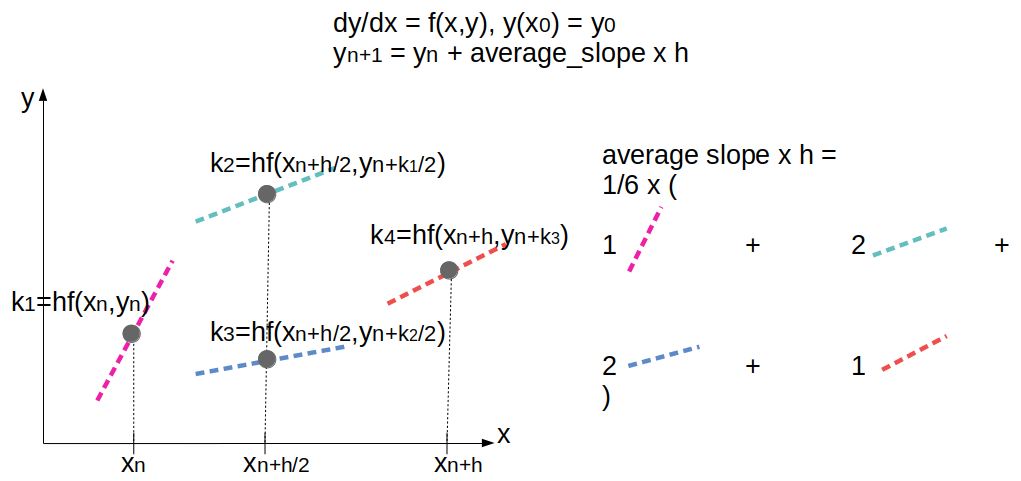
\includegraphics[height=5.5cm]{img/rk/diagram_rk4_slopes.png}
    \caption{RK4 uses a weighted average of four slopes $f(x,y)$ to update $y_n$.}
\end{figure}

Algorithmically, RK4 with the  parameter selection in \eqref{eq:rk4_1_1} to \eqref{eq:rk4_1_4} can be implemented as follows.

\begin{algorithm}[H]
\caption{Runge-Kutta 4th order}
\begin{algorithmic}[1]
\Procedure{RK4} {$f(x,y)$, $[x_0,x_n]$, $f(x_0)$, $h$}
\State $x\leftarrow x_0$
\State $y\leftarrow f(x_0)$
\While {$x < x_n$}
\State $x \leftarrow x + h$
\State $k_1 \leftarrow hf(x,y)$
\State $k_2 \leftarrow hf(x_n + \frac{h}{2}, y_n + \frac{k_1}{2}) $
\State $k_3 \leftarrow hf(x_n + \frac{h}{2}, y_n + \frac{k_2}{2})$
\State $k_4 \leftarrow hf(x_n +h, y_n + k_3)$
\State $y \leftarrow y + \frac{1}{6}\left(k_1 + 2k_2 + 2k_3 + k_4 \right)$ \Comment{$y_{n+1} \leftarrow y_n + \ldots$}
\EndWhile
\EndProcedure
\end{algorithmic}
\label{alg:rk4}
\end{algorithm}

\begin{exmp}
For the initial value problem
\[
\frac{dy}{dx} = y - x^2 + 1, \quad y(0) = 0.5
\]
estimate $y(1.5)$ in steps of $h=0.5$ using the specific RK4 method in \eqref{eq:rk4_1_1} to \eqref{eq:rk4_1_4}.
\end{exmp}

\begin{soln}
By following Alg. \ref{alg:rk4}, we obtain the following values and estimate $y(1.5) \approx 4.0134$.            
                
\begin{tabular}{SSSSSSS} \toprule
    {$x_i$} & {$k_1$} & {$k_2$} & {$k_3$} & {$k_4$} & {$y_n$} & {$y_{n+1}$} \\ \midrule
    0.0 & 0,7500 & 0.9062 & 0.9453 & 1.0976 & 1.0000 & 1.4251 \\
    0.5 & 1.0875 & 1.2032 & 1.2321 & 1.3286 & 1.4251 & 2.6396 \\
    1.0 & 1.3198 & 1.3685 & 1.3806 & 1.4251 & 2.6396 & 4.0134 \\
    1.5 &  &  &  &  & 4.0134 &  \\ \bottomrule
\end{tabular}                
\end{soln}

 
% https://books.google.gr/books?id=FYs1-SGPbrQC&pg=PA461&dq=runge-kutta&hl=en#v=onepage&q=runge-kutta&f=false
% https://www.unf.edu/~mzhan/chapter5.pdf
% https://ocw.snu.ac.kr/sites/default/files/NOTE/Lecture%2010_0.pdf
% https://www.cfm.brown.edu/people/dobrush/am33/Mathematica/ch3/RK4.html
% https://www.math.auckland.ac.nz/~butcher/ODE-book-2008/Tutorials/RK-methods.pdf
% https://www.youtube.com/watch?v=r-jWnXjwQvk&t=14s
% https://www.haroldserrano.com/blog/visualizing-the-runge-kutta-method
% https://wigglewave.wordpress.com/2012/11/09/intuitive-description-of-runge-kutta-integration/
% https://www.intmath.com/differential-equations/12-runge-kutta-rk4-des.php
% https://www.youtube.com/watch?v=pe_m8pfZWcs
% formula only: https://chrishyland.github.io/Runge-Kutta/
%https://digitalcommons.ursinus.edu/cgi/viewcontent.cgi?article=1007&context=triumphs_differ
% https://www.math.auckland.ac.nz/~butcher/CONFERENCES/JAPAN/KYUSHU/kyushu-slides.pdf



% next: https://www.cliffsnotes.com/study-guides/differential-equations/second-order-equations/second-order-homogeneous-equations


%=-=-=-=-=-=-=-=-=-=-=-=-=-=-=-=-=-=-=-=-=-=-=-=-=-=-=-=-=-=-=-=-=-=-=-=-=-=-=-=-
% References
%=-=-=-=-=-=-=-=-=-=-=-=-=-=-=-=-=-=-=-=-=-=-=-=-=-=-=-=-=-=-=-=-=-=-=-=-=-=-=-=-
\newpage
%\printbibliography



%=-=-=-=-=-=-=-=-=-=-=-=-=-=-=-=-=-=-=-=-=-=-=-=-=-=-=-=-=-=-=-=-=-=-=-=-=-=-=-=-
% Appendices
%=-=-=-=-=-=-=-=-=-=-=-=-=-=-=-=-=-=-=-=-=-=-=-=-=-=-=-=-=-=-=-=-=-=-=-=-=-=-=-=-
\newpage
\appendix

\section{Appendices}

% ------------------------ New appendix ------------------------ %
\newpage
\subsection{Lake Pollution Model Solution in Matlab}
\label{app:code_lake_pollution}

\lstinputlisting[language=matlab,caption={A code listing (\detokenize{src/lake_pollution/lake.m)}.}, label=src:mylabel]{src/lake_pollution/lake.m}
The particular solutions \texttt{y} for various initial concentrations \texttt{c0} can be plotted by the following snippet:
\begin{verbatim}
dt = 0.01;
timespan = 0:dt:100;
c0 = 1e6 * [1, 7/3, 11/3, 5]
hold on;

for i = 1:length(c0)
  [_, y] = ode23(@lake, timespan, c0(i));
  plot(t, y);
end

xlabel('t (days)'); ylabal('pol. concentration (kg/m^3)'); grid on;
% reset figure holding and close windows
hold off;
close all;
\end{verbatim}



% ------------------------ New appendix ------------------------ %
\newpage
\subsection{Lake Pollution Model Solution in Matlab}
\label{app:code_slope_field}

\lstinputlisting[language=matlab,caption={A code listing (\detokenize{src/slope_fields/slope_field.m)}.}, label=src:mylabel]{src/slope_fields/slope_field.m}


% ------------------------ New appendix ------------------------ %
\newpage
\subsection{Lake Pollution Model Solution in Matlab}
\label{app:code_eulers_method}

\lstinputlisting[language=matlab,caption={A code listing (\detokenize{src/euler/myeuler.m)}.}, label=src:mylabel]{src/euler/myeuler.m}


\end{document}